% ===========================================================================
%  doc_1/main.tex
%
%  "How the OpenMP engine works, and what in it is new."
%
%  This is NOT a paper.  It is the internal explanation a paper is written
%  FROM: every claim is traced to the source file that implements it, every
%  theoretical claim that is genuinely ours is stated and proved, and every
%  claim that is standard or ported is credited as such.
%
%  Build:  make            (latexmk -pdf main.tex)
%  Layout: one file per section, one file per figure.
% ===========================================================================
\documentclass[11pt,a4paper]{article}
\usepackage[margin=27mm]{geometry}
% ---------------------------------------------------------------------------
%  preamble.tex -- doc_1 : the OpenMP engine explained
%
%  DELIBERATELY MONOCHROME.  Every figure in this document must survive being
%  printed on a black-and-white laser printer and photocopied twice, which is
%  what actually happens to a TACAS submission.  The only "colours" used are
%  greys (black!N) and hatch patterns; nothing carries meaning by hue alone.
% ---------------------------------------------------------------------------
\usepackage[T1]{fontenc}
\usepackage[utf8]{inputenc}
\usepackage{lmodern}
\usepackage{microtype}
\usepackage{amsmath,amssymb,amsthm}
\usepackage{booktabs}
\usepackage{multirow}
\usepackage{array}
\usepackage{graphicx}
\usepackage{caption}
\usepackage{enumitem}
\usepackage{listings}
\usepackage{xcolor}
\usepackage{tikz}
\usepackage{pgfplots}
\pgfplotsset{compat=1.18}
\usetikzlibrary{%
  arrows.meta, positioning, calc, fit, backgrounds,
  shapes.geometric, shapes.misc, decorations.pathreplacing,
  decorations.markings, matrix, patterns, patterns.meta}
\usepackage[hidelinks]{hyperref}
\usepackage[nameinlink,capitalise]{cleveref}

% ---- theorem environments --------------------------------------------------
\theoremstyle{plain}
\newtheorem{theorem}{Theorem}[section]
\newtheorem{lemma}[theorem]{Lemma}
\newtheorem{proposition}[theorem]{Proposition}
\newtheorem{corollary}[theorem]{Corollary}
\theoremstyle{definition}
\newtheorem{definition}[theorem]{Definition}
\newtheorem{example}[theorem]{Example}
\theoremstyle{remark}
\newtheorem{remark}[theorem]{Remark}

% "Intuition" boxes: the same content restated for a reader who does not know
% what a DBM is.  Set apart typographically, never in colour.
\newenvironment{intuition}
  {\par\vspace{2pt}\noindent\begin{list}{}{%
     \setlength{\leftmargin}{1.2em}\setlength{\rightmargin}{0.6em}%
     \setlength{\labelwidth}{0pt}\setlength{\labelsep}{0pt}%
     \setlength{\itemindent}{0pt}\setlength{\listparindent}{0pt}}%
   \item\relax
   \rule{\linewidth}{0.4pt}\par\vspace{2pt}%
   \small\textit{In plain words.}\enspace}
  {\par\vspace{2pt}\rule{\linewidth}{0.4pt}\end{list}\vspace{2pt}}

% ---- monochrome TikZ house style -------------------------------------------
\tikzset{
  >=Stealth,
  node distance=6mm and 8mm,
  bx/.style       = {draw=black, line width=0.5pt, rounded corners=1.5pt,
                     align=center, font=\small, inner sep=4pt,
                     minimum height=7.5mm, fill=white},
  bxs/.style      = {bx, font=\scriptsize, minimum height=6mm, inner sep=3pt},
  tone/.style     = {fill=black!8},
  tonedk/.style    = {fill=black!18},
  hatch/.style    = {pattern=north east lines, pattern color=black!45},
  lane/.style     = {draw=black!45, line width=0.4pt, rounded corners=2pt,
                     dash pattern=on 2pt off 1.5pt, inner sep=5pt},
  fl/.style       = {->, line width=0.55pt, draw=black},
  flt/.style      = {->, line width=0.4pt, draw=black!60},
  fld/.style      = {->, line width=0.5pt, draw=black!70, dashed},
  lbl/.style      = {font=\scriptsize, text=black!75, align=center},
  lblit/.style    = {font=\scriptsize\itshape, text=black!70, align=center},
  tag/.style      = {font=\scriptsize\bfseries, inner sep=1.5pt},
  st/.style       = {circle, draw=black, line width=0.5pt, fill=white,
                     font=\scriptsize, inner sep=1pt, minimum size=5.5mm},
  zn/.style       = {draw=black!70, line width=0.4pt, rounded corners=1pt,
                     fill=white, font=\scriptsize\ttfamily, inner sep=2.5pt,
                     minimum height=4.5mm},
  dead/.style     = {zn, draw=black!35, text=black!45,
                     dash pattern=on 1.5pt off 1.5pt},
  barrier/.style  = {draw=black, line width=1.1pt},
  brace/.style    = {decorate, decoration={brace, amplitude=4pt}, draw=black!60,
                     line width=0.4pt},
}

% ---- listings --------------------------------------------------------------
\lstset{
  basicstyle=\ttfamily\scriptsize,
  breaklines=true, columns=fullflexible, keepspaces=true,
  frame=single, rulecolor=\color{black!35}, framesep=4pt,
  xleftmargin=2pt, showstringspaces=false,
  language=C++,
  commentstyle=\color{black!55}\itshape,
  keywordstyle=\bfseries,
  morekeywords={pragma,omp,parallel,for,schedule,dynamic,nowait,num_threads}
}

% ---- macros ----------------------------------------------------------------
\newcommand{\tool}{\textsc{Ptctlmc}}
\newcommand{\uppaal}{\textsc{Uppaal}}
\newcommand{\ltsmin}{\textsc{LTSmin}}
\newcommand{\opaal}{\textsc{opaal}}
\newcommand{\tchecker}{\textsc{TChecker}}
\newcommand{\code}[1]{\texttt{\small #1}}
\newcommand{\file}[1]{\texttt{\small #1}}

\newcommand{\Clocks}{\mathcal{C}}
\newcommand{\Val}{\mathbb{V}}
\newcommand{\Zn}{Z}
\newcommand{\dk}{\mathit{dk}}
\newcommand{\Cov}{\mathrm{Cov}}
\newcommand{\Post}{\mathit{Post}}
\newcommand{\aLU}{\mathfrak{a}_{LU}}
\newcommand{\subs}{\sqsubseteq}
\newcommand{\extraLU}{\mathit{Extra}^{+}_{LU}}
\newcommand{\hull}{\mathrel{\sqcup}}
\newcommand{\NB}{\mathit{NB}}


% ---- figures: one file each, loaded up front, emitted where wanted --------
% -------------------------------------------------------------------------
%  fig-layers.tex  --  the three storage layers
% -------------------------------------------------------------------------
\newcommand{\FigLayers}{%
\begin{figure}[tb]
\centering
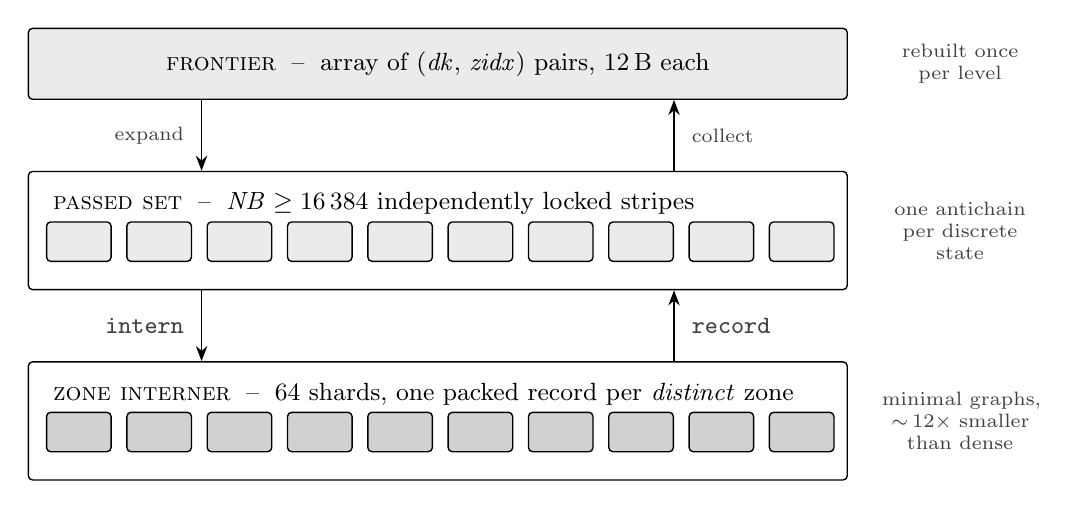
\begin{tikzpicture}

  % ---- frontier -----------------------------------------------------------
  \node[bx, tone, minimum width=104mm, minimum height=9mm] (fr)
    {\textsc{frontier} \;--\; array of $(\dk,\,\mathit{zidx})$ pairs, $12$\,B each};
  \node[lbl, right=2mm of fr.east, anchor=west, text width=22mm]
    {rebuilt once\\per level};

  % ---- passed -------------------------------------------------------------
  \node[bx, below=9mm of fr, minimum width=104mm, minimum height=15mm] (pa) {};
  \node[anchor=north west, font=\small] at ([shift={(2mm,-1.5mm)}]pa.north west)
    {\textsc{passed set} \;--\; $\NB \ge 16\,384$ independently locked stripes};
  \foreach \i in {0,...,9} {
    \node[bxs, tone, minimum width=8.2mm, minimum height=5mm]
      at ([shift={(6.5mm+\i*10.2mm, -9mm)}]pa.north west) {};
  }
  \node[lbl, right=2mm of pa.east, anchor=west, text width=22mm]
    {one antichain\\per discrete\\state};

  % ---- interner -----------------------------------------------------------
  \node[bx, below=9mm of pa, minimum width=104mm, minimum height=15mm] (zi) {};
  \node[anchor=north west, font=\small] at ([shift={(2mm,-1.5mm)}]zi.north west)
    {\textsc{zone interner} \;--\; $64$ shards, one packed record per \emph{distinct} zone};
  \foreach \i in {0,...,9} {
    \node[bxs, tonedk, minimum width=8.2mm, minimum height=5mm]
      at ([shift={(6.5mm+\i*10.2mm, -9mm)}]zi.north west) {};
  }
  \node[lbl, right=2mm of zi.east, anchor=west, text width=22mm]
    {minimal graphs,\\$\sim$\,$12\times$ smaller\\than dense};

  % ---- arrows -------------------------------------------------------------
  \draw[fl] ([xshift=-30mm]fr.south) -- node[lbl,left=1mm]{expand} ([xshift=-30mm]pa.north);
  \draw[fl] ([xshift=30mm]pa.north)  -- node[lbl,right=1mm]{collect} ([xshift=30mm]fr.south);
  \draw[fl] ([xshift=-30mm]pa.south) -- node[lbl,left=1mm]{\code{intern}} ([xshift=-30mm]zi.north);
  \draw[fl] ([xshift=30mm]zi.north)  -- node[lbl,right=1mm]{\code{record}} ([xshift=30mm]pa.south);

\end{tikzpicture}
\caption{The three storage layers of the OpenMP engine and the traffic between
them.  Nothing in the engine holds a symbolic state as an object: the frontier
holds a packed discrete key plus a $4$-byte zone index, the passed set holds
antichains of zone indices, and only the interner holds zone \emph{bytes} --
once per distinct zone, in minimal-graph form.  The layering is what makes the
resident working set small enough to stay in cache while $32$ threads hammer
it.}
\label{fig:layers}
\end{figure}}

% -------------------------------------------------------------------------
%  fig-level.tex  --  one BFS level: phases, barrier, ragged tail
%
%  Layout budget (mm, x=1mm y=1mm).  Keep boxes at FIXED text width so a long
%  label cannot silently widen a node and collide with its neighbour.
%     x  -8 .. 74   expand phase + thread lanes        x 74  barrier
%     x  78 .. 140  the three post-barrier phases
%     y  20         phase row      y 13..7  sub-captions
%     y   0 .. -15  thread lanes   y -20    tail-idle brace
%     y -30         feedback edge
% -------------------------------------------------------------------------
\newcommand{\FigLevel}{%
\begin{figure}[tb]
\centering
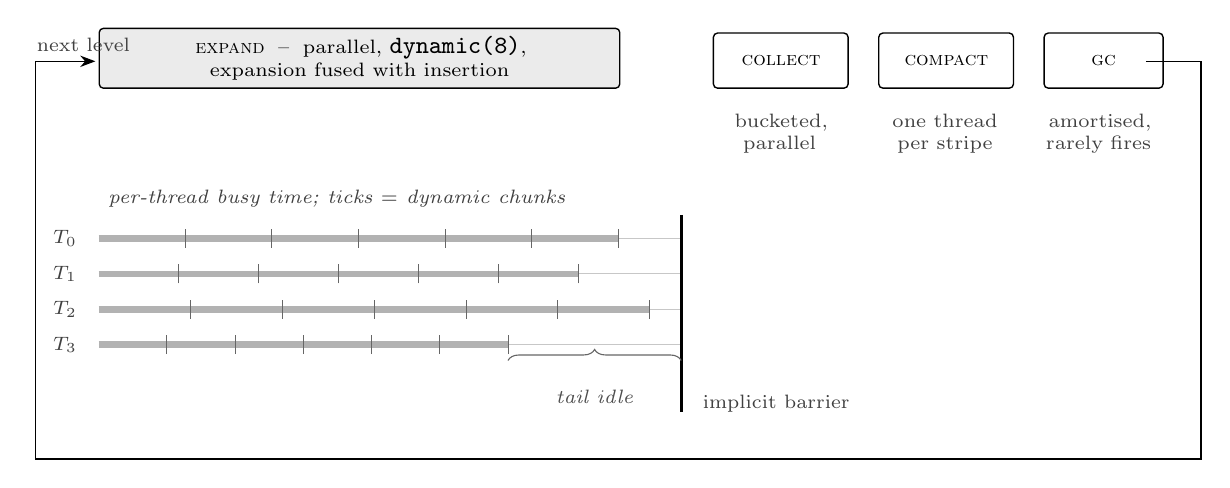
\begin{tikzpicture}[x=1mm,y=1mm]

  % ---- phase row --------------------------------------------------------
  \node[bxs, tone, anchor=south west, text width=64mm, align=center,
        minimum height=7mm] (ph) at (0,17)
    {\textsc{expand} \;--\; parallel, \code{dynamic(8)},\\
     expansion fused with insertion};

  \node[bxs, anchor=south west, text width=15mm, align=center, minimum height=7mm]
    (c1) at (78,17) {\textsc{collect}};
  \node[bxs, anchor=south west, text width=15mm, align=center, minimum height=7mm]
    (c2) at (99,17) {\textsc{compact}};
  \node[bxs, anchor=south west, text width=13mm, align=center, minimum height=7mm]
    (c3) at (120,17) {\textsc{gc}};

  \node[lbl, anchor=north, text width=20mm] at (86.5,15) {bucketed,\\parallel};
  \node[lbl, anchor=north, text width=20mm] at (107.5,15){one thread\\per stripe};
  \node[lbl, anchor=north, text width=18mm] at (127,15)  {amortised,\\rarely fires};

  % ---- thread lanes -----------------------------------------------------
  % \len marks where a worker runs out of chunks; the spread is the tail.
  \node[lbl, anchor=west] at (0,3) {\itshape per-thread busy time; ticks $=$ dynamic chunks};
  \foreach \t/\len in {0/66, 1/61, 2/70, 3/52} {
    \pgfmathsetmacro\yy{-2-\t*4.5}
    \node[lbl, anchor=east] at (-1.5,\yy) {$T_\t$};
    \draw[draw=black!22, line width=0.4pt] (0,\yy) -- (74,\yy);
    \draw[line width=2.4pt, draw=black!30] (0,\yy) -- (\len,\yy);
    \foreach \c in {1,...,6} {
      \pgfmathsetmacro\xx{\c*(\len/6)}
      \draw[draw=black!60, line width=0.35pt] (\xx,\yy-1.2) -- (\xx,\yy+1.2);
    }
  }

  % ---- barrier ----------------------------------------------------------
  \draw[barrier] (74,1) -- (74,-24);
  \node[lbl, anchor=west] at (75.5,-23) {implicit barrier};

  % ---- tail idle --------------------------------------------------------
  \draw[brace] (52,-17.5) -- (74,-17.5);
  \node[lblit, anchor=north] at (63,-20) {tail idle};

  % ---- feedback edge ----------------------------------------------------
  \draw[fl] (133,20.5) -- (140,20.5) -- (140,-30) -- (-8,-30) -- (-8,20.5)
            -- node[lbl, above, pos=0.8] {next level} (-0.4,20.5);

\end{tikzpicture}
\caption{Anatomy of one BFS level.  \textsc{expand} is the only phase that
touches the transition relation and the only one that runs for a long time; the
three phases after the barrier exist purely to keep memory bounded.  The tick
marks are dynamic-schedule chunks: because a chunk is only $8$ frontier states,
the lanes finish close together and the leftover \emph{tail idle} is small --
it is the price of level-synchronous BFS, paid deliberately in exchange for a
smaller state space.  Every phase after the barrier was itself parallelised or
given an amortised trigger, because by Amdahl's law each one caps the
achievable speedup independently of the others.}
\label{fig:level}
\end{figure}}

% -------------------------------------------------------------------------
%  fig-stripes.tex  --  the striped passed set
% -------------------------------------------------------------------------
\newcommand{\FigStripes}{%
\begin{figure}[tb]
\centering
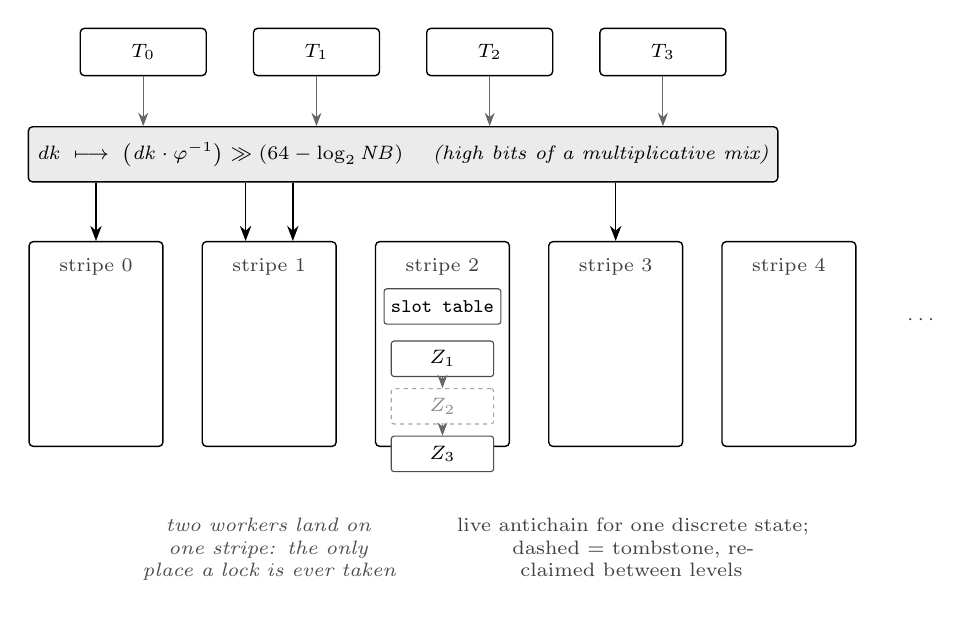
\begin{tikzpicture}[x=1mm,y=1mm]

  % threads
  \foreach \t/\x in {0/0, 1/22, 2/44, 3/66} {
    \node[bxs, minimum width=16mm] (T\t) at (\x,0) {$T_\t$};
  }

  % hash box
  \node[bxs, tone, minimum width=88mm, minimum height=7mm] (h) at (33,-13)
    {$\dk \;\longmapsto\; \big(\dk \cdot \varphi^{-1}\big) \gg (64-\log_2 \NB)$
     \quad\textit{(high bits of a multiplicative mix)}};

  \foreach \t in {0,...,3} { \draw[flt] (T\t) -- (T\t |- h.north); }

  % stripes
  \foreach \s/\x in {0/-6, 1/16, 2/38, 3/60, 4/82} {
    \node[bxs, minimum width=17mm, minimum height=26mm, anchor=north] (S\s) at (\x,-24) {};
    \node[lbl, anchor=north] at ([yshift=-1mm]S\s.north) {stripe \s};
  }
  \node[lbl] at (99,-34) {$\cdots$};

  % contents of one stripe, drawn in stripe 2
  \node[zn, anchor=north, minimum width=13mm] (slot) at ([yshift=-6mm]S2.north)
    {slot table};
  \node[zn, anchor=north, minimum width=13mm] (a1) at ([yshift=-2mm]slot.south) {$Z_1$};
  \node[dead, anchor=north, minimum width=13mm] (a2) at ([yshift=-1.4mm]a1.south) {$Z_2$};
  \node[zn, anchor=north, minimum width=13mm] (a3) at ([yshift=-1.4mm]a2.south) {$Z_3$};
  \draw[flt] (a1) -- (a2);  \draw[flt] (a2) -- (a3);

  % arrows from hash to stripes: two threads collide on stripe 1
  \draw[fl] (h.south -| S0) -- (S0.north);
  \draw[fl] ([xshift=-3mm]h.south -| S1) -- ([xshift=-3mm]S1.north);
  \draw[fl] ([xshift=3mm]h.south -| S1)  -- ([xshift=3mm]S1.north);
  \draw[fl] (h.south -| S3) -- (S3.north);

  \node[lblit, anchor=north, text width=44mm] at (16,-58)
    {two workers land on one stripe: the only\\place a lock is ever taken};

  \node[lbl, anchor=north, text width=48mm] at (62,-58)
    {live antichain for one discrete state;\\dashed $=$ tombstone, reclaimed between levels};

\end{tikzpicture}
\caption{The passed set is one flat table split into $\NB \ge 16\,384$
independently locked stripes.  A discrete state's key $\dk$ selects its stripe
by the \emph{high} bits of a multiplicative hash; within a stripe an
open-addressed slot table maps $\dk$ to the head of a linked antichain of zone
indices.  There is no static partition of the state space among threads --
any worker may write any stripe -- so no worker can be starved by an unlucky
partition, and there is no routing barrier between expansion and insertion.
With $\NB \gg$ threads, two workers colliding on the same stripe is rare
(measured $2$--$3\%$); \cref{fig:protocol} explains why even a collision is
usually cheap.}
\label{fig:stripes}
\end{figure}}

% -------------------------------------------------------------------------
%  fig-protocol.tex  --  the two-phase lock protocol
%
%  A straight top-to-bottom spine (successor -> phase 1 -> phase 2) with the
%  two exits leaving to the RIGHT at their own heights, so no edge label can
%  collide with a box.  Annotations live to the right of the exits.
% -------------------------------------------------------------------------
\newcommand{\FigProtocol}{%
\begin{figure}[tb]
\centering
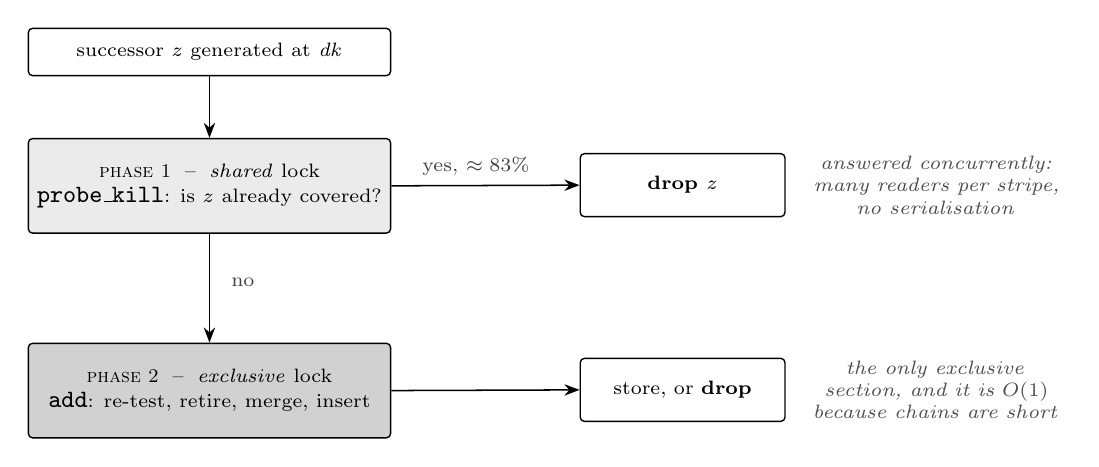
\begin{tikzpicture}[x=1mm,y=1mm]

  % ---- spine ------------------------------------------------------------
  \node[bxs, anchor=north, minimum width=46mm] (s) at (25,0)
    {successor $z$ generated at $\dk$};

  \node[bxs, tone, anchor=north, minimum width=46mm, minimum height=12mm]
    (p) at (25,-14)
    {\textsc{phase 1} \;--\; \emph{shared} lock\\[1pt]
     \code{probe\_kill}: is $z$ already covered?};

  \node[bxs, tonedk, anchor=north, minimum width=46mm, minimum height=12mm]
    (x) at (25,-40)
    {\textsc{phase 2} \;--\; \emph{exclusive} lock\\[1pt]
     \code{add}: re-test, retire, merge, insert};

  \draw[fl] (s.south) -- (p.north);
  \draw[fl] (p.south) -- node[lbl, right=1.5mm, pos=0.45] {no} (x.north);

  % ---- exits ------------------------------------------------------------
  \node[bxs, anchor=west, minimum width=26mm, minimum height=8mm] (drop) at (72,-20)
    {\textbf{drop $z$}};
  \node[bxs, anchor=west, minimum width=26mm, minimum height=8mm] (keep) at (72,-46)
    {store, or \textbf{drop}};

  \draw[fl] (p.east) -- node[lbl, above, pos=0.45] {yes, $\approx 83\%$} (drop.west);
  \draw[fl] (x.east) -- node[lbl, above, pos=0.45] {} (keep.west);

  % ---- annotations ------------------------------------------------------
  \node[lblit, anchor=west, text width=32mm] at (100,-20)
    {answered concurrently:\\many readers per stripe,\\no serialisation};
  \node[lblit, anchor=west, text width=32mm] at (100,-46)
    {the only exclusive\\section, and it is $O(1)$\\because chains are short};

\end{tikzpicture}
\caption{The two-phase stripe protocol.  Phase~1 is exactly the read-only
prefix of the insertion procedure, run under a \emph{shared} lock: on
\code{phil13} it disposes of $83\%$ of all $23$\,M insertion attempts, and
because shared locks do not exclude each other, those $83\%$ never serialise.
Phase~2 re-runs the test under an exclusive lock, so a stale ``no'' from
phase~1 costs one wasted lock acquisition and can never change the outcome.  A
stale ``yes'' \emph{would} change the outcome ---
\cref{thm:coverage,cor:probe} prove that a ``yes'' can never go stale, which is
what licenses releasing the lock between the two phases.}
\label{fig:protocol}
\end{figure}}

% -------------------------------------------------------------------------
%  fig-add.tex  --  the five steps of add()
% -------------------------------------------------------------------------
\newcommand{\FigAdd}{%
\begin{figure}[tb]
\centering
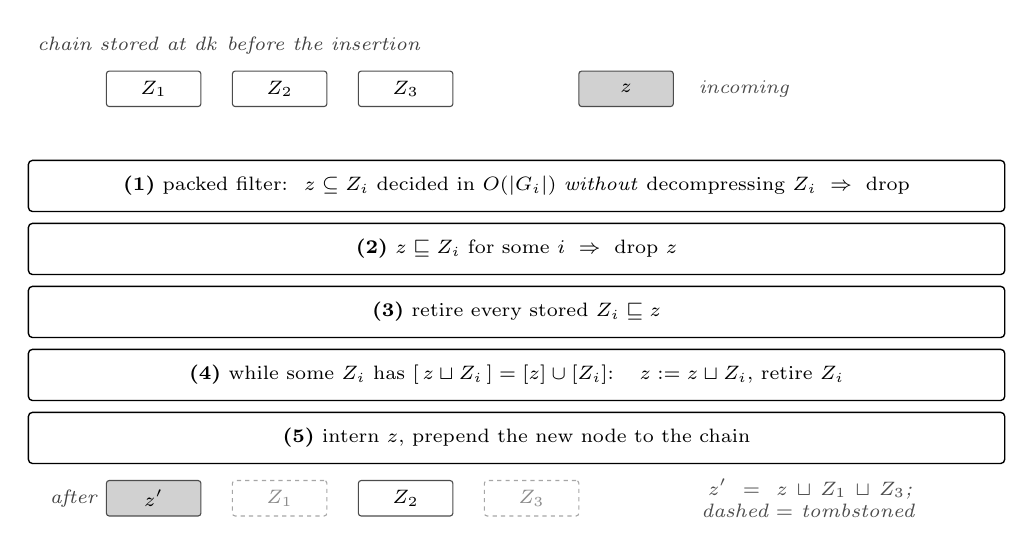
\begin{tikzpicture}[x=1mm,y=1mm]

  \node[lbl, anchor=west] at (-16,5.5) {\itshape chain stored at $\dk$ before the insertion};
  \foreach \i/\n in {0/Z_1, 1/Z_2, 2/Z_3} {
    \pgfmathsetmacro\xx{\i*16}
    \node[zn, minimum width=12mm] (b\i) at (\xx,0) {$\n$};
  }
  \node[zn, tonedk, minimum width=12mm] (zin) at (60,0) {$z$};
  \node[lblit, anchor=west] at (68,0) {incoming};

  % steps
  \node[bxs, anchor=north west, minimum width=124mm, minimum height=6.5mm] (s1) at (-16,-9)
    {\textbf{(1)} packed filter: $\;z \subseteq Z_i$ decided in $O(|G_i|)$ \emph{without} decompressing $Z_i$ \;$\Rightarrow$\; drop};
  \node[bxs, anchor=north west, minimum width=124mm, minimum height=6.5mm] (s2) at (-16,-17)
    {\textbf{(2)} $z \subs Z_i$ for some $i$ \;$\Rightarrow$\; drop $z$};
  \node[bxs, anchor=north west, minimum width=124mm, minimum height=6.5mm] (s3) at (-16,-25)
    {\textbf{(3)} retire every stored $Z_i \subs z$};
  \node[bxs, anchor=north west, minimum width=124mm, minimum height=6.5mm] (s4) at (-16,-33)
    {\textbf{(4)} while some $Z_i$ has $[\,z \sqcup Z_i\,] = [z] \cup [Z_i]$: \; $z := z \sqcup Z_i$, retire $Z_i$};
  \node[bxs, anchor=north west, minimum width=124mm, minimum height=6.5mm] (s5) at (-16,-41)
    {\textbf{(5)} intern $z$, prepend the new node to the chain};

  \node[lbl, anchor=east] at (-6,-52) {\itshape after};
  \node[zn, tonedk, minimum width=12mm] (a0) at (0,-52) {$z'$};
  \node[dead, minimum width=12mm] (a1) at (16,-52) {$Z_1$};
  \node[zn, minimum width=12mm] (a2) at (32,-52) {$Z_2$};
  \node[dead, minimum width=12mm] (a3) at (48,-52) {$Z_3$};
  \node[lblit, anchor=west, text width=44mm] at (60,-52)
    {$z' = z \sqcup Z_1 \sqcup Z_3$;\\dashed $=$ tombstoned};

\end{tikzpicture}
\caption{Insertion into one discrete state's antichain.  Steps (2) and (3)
are the classical subsumption test in both directions.  Step (4) is the
\emph{exact} convex-union merge: if the convex hull of two zones happens to
contain no point outside their union, the two are replaced by the hull with no
loss of precision (\cref{thm:hull}).  Step (4) is what keeps chains at
$\approx 1$ zone per discrete state on every process network we measure, which
in turn is what makes the critical section in \cref{fig:protocol} $O(1)$ rather
than $O(\text{chain})$.  Step (1) is a pure optimisation of step (2) that runs
directly on the compressed representation -- see \cref{fig:mingraph}.}
\label{fig:add}
\end{figure}}

% -------------------------------------------------------------------------
%  fig-hull.tex  --  geometry of the convex-union test
% -------------------------------------------------------------------------
\newcommand{\FigHull}{%
\begin{figure}[tb]
\centering
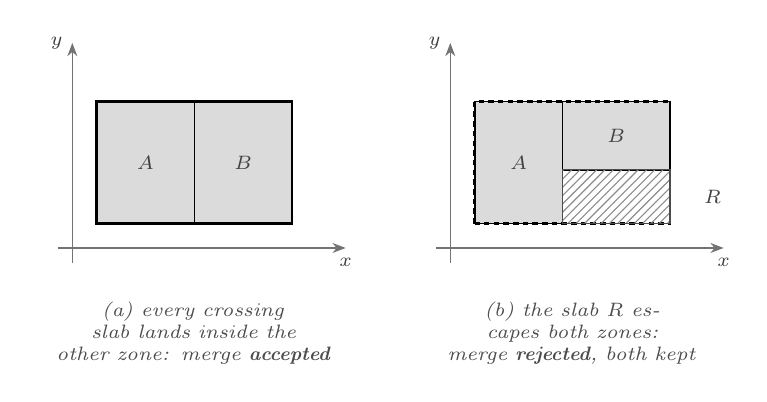
\begin{tikzpicture}[x=6.2mm,y=6.2mm]

% ---------- panel (a): union is convex ----------
\begin{scope}
  \draw[->, black!55, line width=0.4pt] (-0.3,0) -- (5.6,0) node[lbl, below]{$x$};
  \draw[->, black!55, line width=0.4pt] (0,-0.3) -- (0,4.2) node[lbl, left]{$y$};
  \fill[black!14] (0.5,0.5) rectangle (2.5,3.0);
  \fill[black!14] (2.5,0.5) rectangle (4.5,3.0);
  \draw[black, line width=0.6pt] (0.5,0.5) rectangle (2.5,3.0);
  \draw[black, line width=0.6pt] (2.5,0.5) rectangle (4.5,3.0);
  \draw[black, line width=1.0pt] (0.5,0.5) rectangle (4.5,3.0);
  \node[lbl] at (1.5,1.75) {$A$};
  \node[lbl] at (3.5,1.75) {$B$};
  \node[lblit, anchor=north, text width=40mm] at (2.5,-0.9)
    {(a) every crossing slab lands inside the\\other zone: merge \textbf{accepted}};
\end{scope}

% ---------- panel (b): union is not convex ----------
\begin{scope}[xshift=48mm]
  \draw[->, black!55, line width=0.4pt] (-0.3,0) -- (5.6,0) node[lbl, below]{$x$};
  \draw[->, black!55, line width=0.4pt] (0,-0.3) -- (0,4.2) node[lbl, left]{$y$};
  \fill[black!14] (0.5,0.5) rectangle (2.3,3.0);
  \fill[black!14] (2.3,1.6) rectangle (4.5,3.0);
  \draw[black, line width=0.6pt] (0.5,0.5) rectangle (2.3,3.0);
  \draw[black, line width=0.6pt] (2.3,1.6) rectangle (4.5,3.0);
  \draw[black, line width=1.0pt, dash pattern=on 2pt off 1.5pt]
    (0.5,0.5) rectangle (4.5,3.0);
  % the escaping crossing region
  \fill[hatch] (2.3,0.5) rectangle (4.5,1.6);
  \draw[black!70, line width=0.4pt] (2.3,0.5) rectangle (4.5,1.6);
  \node[lbl] at (1.4,1.75) {$A$};
  \node[lbl] at (3.4,2.3) {$B$};
  \node[lbl, anchor=west] at (5.0,1.05) {$R$};
  \node[lblit, anchor=north, text width=40mm] at (2.5,-0.9)
    {(b) the slab $R$ escapes both zones:\\merge \textbf{rejected}, both kept};
\end{scope}

\end{tikzpicture}
\caption{The convex-union test, in two clocks.  The hull $A \sqcup B$ is the
entrywise-loosest DBM.  For every facet of $A$ that is \emph{strictly} inside
the hull, the algorithm computes the slab $R$ of the hull lying on the far side
of that facet, and demands $R \subseteq B$ (and symmetrically).  In (a) every
such slab is inside the other zone and the hull is exactly the union, so the
two zones collapse into one with no loss.  In (b) the slab $R$ contains points
in neither $A$ nor $B$, so the hull would add unreachable valuations and the
merge is refused.  \cref{thm:hull} shows the test is not a heuristic: it
accepts \emph{exactly} the pairs whose union is convex.}
\label{fig:hull}
\end{figure}}

% -------------------------------------------------------------------------
%  fig-mingraph.tex  --  dense DBM vs minimal graph, and the O(|G|) inclusion test
% -------------------------------------------------------------------------
\newcommand{\FigMingraph}{%
\begin{figure}[tb]
\centering
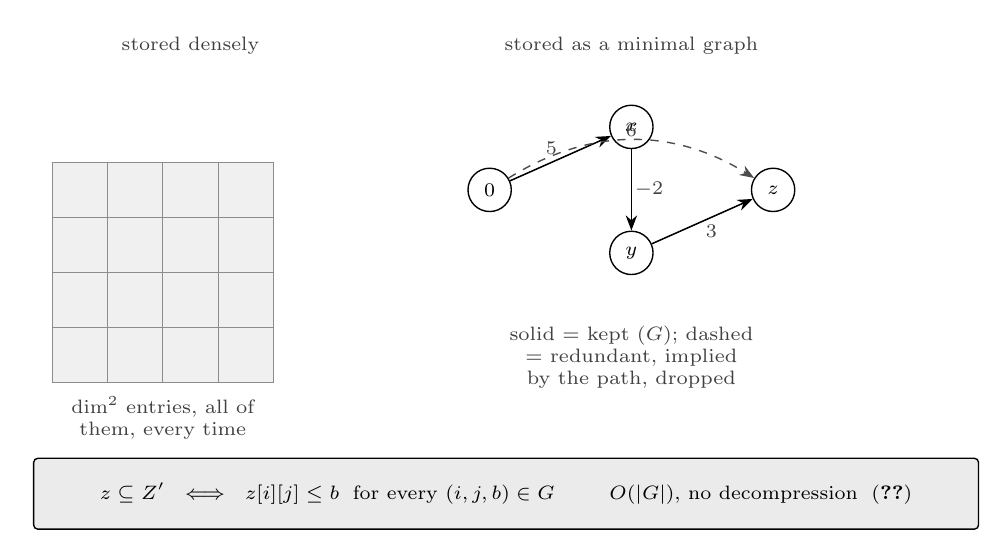
\begin{tikzpicture}[x=1mm,y=1mm]

% ---- dense -----------------------------------------------------------------
\begin{scope}
  \node[lbl, anchor=south] at (14,16) {stored densely};
  \foreach \i in {0,...,3} \foreach \j in {0,...,3} {
    \pgfmathsetmacro\xx{\j*7}
    \pgfmathsetmacro\yy{-\i*7}
    \node[draw=black!45, line width=0.3pt, fill=black!6,
          minimum width=7mm, minimum height=7mm, inner sep=0pt] at (\xx,\yy) {};
  }
  \node[lbl, anchor=north, text width=32mm] at (10.5,-25)
    {$\dim^2$ entries, all of them, every time};
\end{scope}

% ---- minimal graph ---------------------------------------------------------
\begin{scope}[xshift=52mm]
  \node[lbl, anchor=south] at (18,16) {stored as a minimal graph};
  \node[st] (x0) at (0,0)   {$0$};
  \node[st] (x1) at (18,8)  {$x$};
  \node[st] (x2) at (18,-8) {$y$};
  \node[st] (x3) at (36,0)  {$z$};
  \draw[fl] (x0) -- node[lbl,above left,inner sep=1pt]{$5$}  (x1);
  \draw[fl] (x1) -- node[lbl,right,inner sep=1pt]{$-2$} (x2);
  \draw[fl] (x2) -- node[lbl,below right,inner sep=1pt]{$3$} (x3);
  \draw[fld, bend left=32] (x0) to node[lbl,above,inner sep=1pt]{$6$} (x3);
  \node[lbl, anchor=north, text width=42mm] at (18,-16)
    {solid $=$ kept ($G$); dashed $=$ redundant, implied by the path, dropped};
\end{scope}

% ---- the test --------------------------------------------------------------
\node[bxs, tone, anchor=north west, minimum width=120mm, minimum height=9mm] (t)
  at (-6,-34)
  {$z \subseteq Z'$ \;$\iff$\; $z[i][j] \le b$ \;for every $(i,j,b) \in G$
   \hspace{6mm}$O(|G|)$, no decompression \;(\cref{lem:mingraph})};

\end{tikzpicture}
\caption{Zones are \emph{operated on} densely and \emph{stored} minimally.  A
canonical DBM is a shortest-path closure, so most of its entries are implied by
the others; the minimal graph keeps only the non-redundant edges, which is
$\approx 144$\,B instead of $1764$\,B for a $21$-clock zone.  The payoff is not
only memory: the inclusion test $z \subseteq Z'$ can be decided directly on the
compressed form in $O(|G|)$, whereas a dense comparison would first have to run
an $O(\dim^3)$ closure to rebuild the redundant entries.  On \code{arbiter17}
that decompression was $36.3$\,s of work feeding $1.6$\,s of comparisons --
$22\times$ more time unpacking a zone than comparing against it.}
\label{fig:mingraph}
\end{figure}}

% -------------------------------------------------------------------------
%  fig-intern.tex  --  the sharded zone interner
% -------------------------------------------------------------------------
\newcommand{\FigIntern}{%
\begin{figure}[tb]
\centering
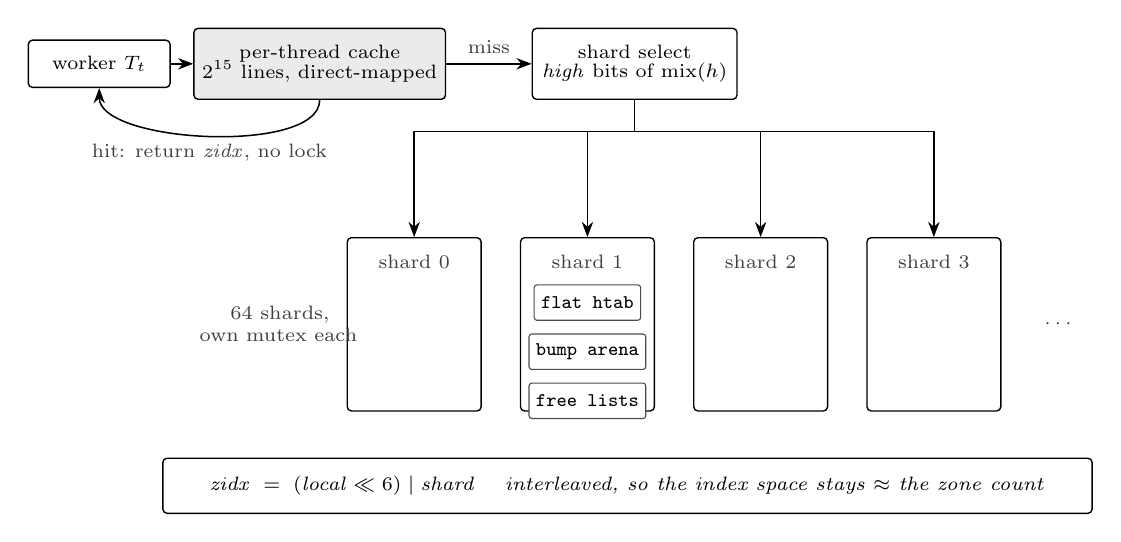
\begin{tikzpicture}[x=1mm,y=1mm]

  \node[bxs, minimum width=18mm] (t) at (0,0) {worker $T_t$};
  \node[bxs, tone, minimum width=30mm, minimum height=9mm] (c) at (28,0)
    {per-thread cache\\[-1pt]\scriptsize $2^{15}$ lines, direct-mapped};
  \node[bxs, minimum width=26mm, minimum height=9mm] (sel) at (68,0)
    {shard select\\[-1pt]\scriptsize \emph{high} bits of mix$(h)$};

  \draw[fl] (t) -- (c);
  \draw[fl] (c) -- node[lbl,above]{miss} (sel);
  \draw[fl] (c.south) .. controls +(0,-7) and +(0,-7) .. (t.south);
  \node[lbl, anchor=north] at (14,-9) {hit: return $\mathit{zidx}$, no lock};

  \foreach \s/\x in {0/40, 1/62, 2/84, 3/106} {
    \node[bxs, minimum width=17mm, minimum height=22mm, anchor=north] (S\s) at (\x,-22) {};
    \node[lbl, anchor=north] at ([yshift=-1mm]S\s.north) {shard \s};
  }
  \node[lbl] at (122,-33) {$\cdots$};
  \node[lbl, anchor=east, text width=20mm] at (34,-33) {$64$ shards,\\own mutex each};

  \node[zn, anchor=north, minimum width=13mm] (h1) at ([yshift=-6mm]S1.north) {flat htab};
  \node[zn, anchor=north, minimum width=13mm] (h2) at ([yshift=-1.6mm]h1.south) {bump arena};
  \node[zn, anchor=north, minimum width=13mm] (h3) at ([yshift=-1.6mm]h2.south) {free lists};

  \draw[fl] (sel.south) -- ++(0,-4) -| (S0.north);
  \draw[fl] (sel.south) -- ++(0,-4) -| (S1.north);
  \draw[fl] (sel.south) -- ++(0,-4) -| (S2.north);
  \draw[fl] (sel.south) -- ++(0,-4) -| (S3.north);

  \node[bxs, anchor=north west, minimum width=118mm, minimum height=7mm] (enc) at (8,-50)
    {$\mathit{zidx} \;=\; (\mathit{local} \ll 6)\;|\;\mathit{shard}$
     \quad\textit{interleaved, so the index space stays $\approx$ the zone count}};

\end{tikzpicture}
\caption{The zone interner.  A zone is packed, hashed, looked up in a
lock-free per-thread cache, and only on a miss routed to one of $64$
independently locked shards.  Two details are load-bearing.  First, the shard
selector must take the \emph{high} bits of a re-mixed hash: if it reused the
low bits that also index a shard's hash table, only $1/64$ of that table's
slots could ever be a home position and probe chains collapse (measured: $31.2$
probes per lookup versus $1.68$).  Second, the index is interleaved rather than
concatenated, so the largest handed-out index stays proportional to the number
of zones -- which is what the garbage collector's mark array is sized by.}
\label{fig:intern}
\end{figure}}

% -------------------------------------------------------------------------
%  fig-coverage.tex  --  coverage monotonicity
%
%  Two panels.  Left: the covered region at time t, and a successor z sitting
%  inside it.  Right: after an update that RETIRES Z_1 -- the retired blob is
%  drawn dashed, strictly inside the blob that replaced it, so the eye sees
%  immediately that coverage grew rather than moved.  Labels are placed OUTSIDE
%  the blobs so nothing overlaps.
% -------------------------------------------------------------------------
\newcommand{\FigCoverage}{%
\begin{figure}[tb]
\centering
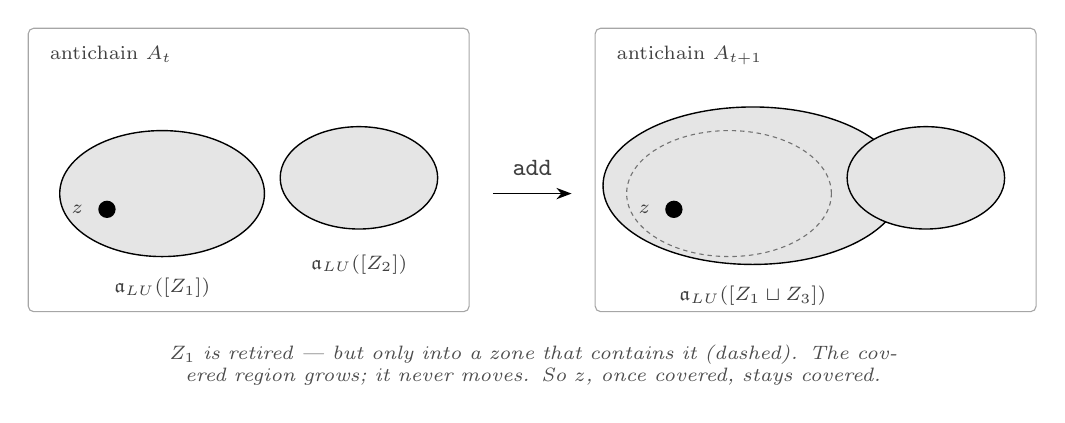
\begin{tikzpicture}[x=1mm,y=1mm]

% ---- panel: time t ------------------------------------------------------
\begin{scope}
  \draw[draw=black!35, line width=0.4pt, rounded corners=2pt]
    (0,-26) rectangle (56,10);
  \node[lbl, anchor=north west] at (1.5,9) {antichain $A_t$};

  \fill[black!10] (17,-11) ellipse (13 and 8);
  \draw[black, line width=0.5pt] (17,-11) ellipse (13 and 8);
  \node[lbl, anchor=north] at (17,-20.5) {$\aLU([Z_1])$};

  \fill[black!10] (42,-9) ellipse (10 and 6.5);
  \draw[black, line width=0.5pt] (42,-9) ellipse (10 and 6.5);
  \node[lbl, anchor=north] at (42,-17.5) {$\aLU([Z_2])$};

  \fill[black] (10,-13) circle (1.1);
  \node[lbl, anchor=east] at (8.2,-13) {$z$};
\end{scope}

% ---- transition ---------------------------------------------------------
\draw[fl] (59,-11) -- (69,-11);
\node[lbl, anchor=south] at (64,-10) {\code{add}};

% ---- panel: time t+1 ----------------------------------------------------
\begin{scope}[xshift=72mm]
  \draw[draw=black!35, line width=0.4pt, rounded corners=2pt]
    (0,-26) rectangle (56,10);
  \node[lbl, anchor=north west] at (1.5,9) {antichain $A_{t+1}$};

  \fill[black!10] (20,-10) ellipse (19 and 10);
  \draw[black, line width=0.5pt] (20,-10) ellipse (19 and 10);
  % the retired zone, drawn where it was: strictly inside its replacement
  \draw[black!55, line width=0.4pt, dash pattern=on 1.6pt off 1.4pt]
    (17,-11) ellipse (13 and 8);
  \node[lbl, anchor=north] at (20,-21.5) {$\aLU([Z_1 \sqcup Z_3])$};

  \fill[black!10] (42,-9) ellipse (10 and 6.5);
  \draw[black, line width=0.5pt] (42,-9) ellipse (10 and 6.5);

  \fill[black] (10,-13) circle (1.1);
  \node[lbl, anchor=east] at (8.2,-13) {$z$};
\end{scope}

\node[lblit, anchor=north, text width=124mm] at (64,-29)
  {$Z_1$ is retired --- but only into a zone that contains it (dashed).  The
   covered region grows; it never moves.  So $z$, once covered, stays covered.};

\end{tikzpicture}
\caption{Coverage monotonicity (\cref{thm:coverage}).  Concurrent workers
mutate an antichain while other workers read it, which is normally fatal to a
lock-free read.  It is safe here because of a structural property of the update
rule: a stored zone is retired only by subsumption or by absorption into a
convex hull, and in both cases the zone that replaces it \emph{contains} it.
The union of the covered regions is therefore non-decreasing over time, so a
``$z$ is already covered'' answer computed under a shared lock cannot be
invalidated by a writer that acquires the lock a nanosecond later.}
\label{fig:coverage}
\end{figure}}

% -------------------------------------------------------------------------
%  fig-scaling.tex  --  measured thread scaling
%
%  MONOCHROME: every \addplot carries an explicit black stroke and is
%  distinguished by mark shape plus dash pattern.  Do NOT use \addplot+ here --
%  the "+" appends pgfplots' default cycle list, which is coloured.
% -------------------------------------------------------------------------
\newcommand{\FigScaling}{%
\begin{figure}[tb]
\centering
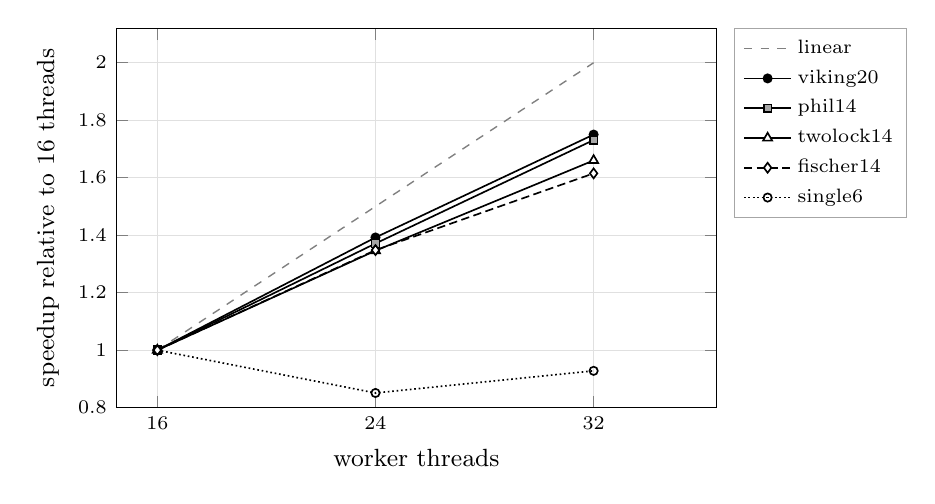
\begin{tikzpicture}
\begin{axis}[
  width=92mm, height=64mm,
  xlabel={worker threads},
  ylabel={speedup relative to $16$ threads},
  xtick={16,24,32}, xmin=14.5, xmax=36.5, ymin=0.8, ymax=2.12,
  ytick={0.8,1.0,1.2,1.4,1.6,1.8,2.0},
  grid=major, grid style={black!12, line width=0.3pt},
  tick label style={font=\scriptsize},
  label style={font=\small},
  legend style={font=\scriptsize, draw=black!35, fill=white,
                at={(1.03,1.0)}, anchor=north west, cells={anchor=west},
                row sep=0.4pt},
  legend cell align=left,
]
\addplot[black!50, dashed, line width=0.5pt, mark=none]
  coordinates {(16,1.0) (24,1.5) (32,2.0)};       \addlegendentry{linear}
\addplot[black, line width=0.6pt, mark=*, mark size=1.5pt,
         mark options={fill=black}]
  coordinates {(16,1.000) (24,1.392) (32,1.750)}; \addlegendentry{viking20}
\addplot[black, line width=0.6pt, mark=square*, mark size=1.4pt,
         mark options={fill=black!35}]
  coordinates {(16,1.000) (24,1.371) (32,1.731)}; \addlegendentry{phil14}
\addplot[black, line width=0.6pt, mark=triangle*, mark size=1.9pt,
         mark options={fill=white}]
  coordinates {(16,1.000) (24,1.346) (32,1.660)}; \addlegendentry{twolock14}
\addplot[black, line width=0.6pt, dash pattern=on 3pt off 1.6pt,
         mark=diamond*, mark size=1.8pt, mark options={solid, fill=white}]
  coordinates {(16,1.000) (24,1.348) (32,1.615)}; \addlegendentry{fischer14}
\addplot[black, line width=0.6pt, densely dotted, mark=o, mark size=1.5pt,
         mark options={solid}]
  coordinates {(16,1.000) (24,0.851) (32,0.928)}; \addlegendentry{single6}
\end{axis}
\end{tikzpicture}
\caption{Measured scaling from $16$ to $32$ workers on the large instances of
each family (wall-clock, best of two runs, \code{--omp-chunk 8}).  Doubling the
worker count buys $1.62$--$1.75\times$, i.e.\ $81$--$87\%$ parallel efficiency
in that range, on every family whose state space is spread over many discrete
states.  \code{single6} is the deliberate counterexample: it is a single
automaton with one location and $N$ independent clocks, so its \emph{entire}
passed set is one discrete state -- one stripe, one antichain, one lock -- and
no amount of hardware helps.  That is a property of the model, not of the
implementation, and it is the honest boundary of this design.}
\label{fig:scaling}
\end{figure}}


\title{\Large The \tool{} OpenMP Engine\\[2pt]
       \large Algorithm, Architecture, and What Is Actually New}
\author{}
\date{}

\begin{document}
\maketitle
\vspace{-10mm}

% ---------------------------------------------------------------------------
%  00-how-to-read.tex -- orientation for the two audiences this document has
% ---------------------------------------------------------------------------
\section*{How to read this document}
\addcontentsline{toc}{section}{How to read this document}

This document has two readers in mind at once, and it tries not to compromise
for either.

\begin{itemize}[leftmargin=1.2em, itemsep=2pt]
\item \textbf{The reader who does not do timed automata.}  Every section opens
      with the idea in ordinary language, and wherever the technical text gets
      dense there is an \emph{In plain words} box restating the same content
      with no notation.  You can read only the opening paragraphs, the boxes,
      and the figure captions and come away with an accurate picture.

\item \textbf{The reader who will referee this.}  The formal statements,
      proofs, and the exact boundary between ``ours'' and ``standard'' are in
      \cref{sec:theory} and \cref{sec:novelty}.  \cref{sec:novelty} is
      deliberately blunt: it lists what is new, what is a port of somebody
      else's idea, and what is engineering that carries no theoretical claim.
      If you only read one section, read that one.
\end{itemize}

\paragraph{Everything is traced to code.}
Each mechanism names the file and the function that implements it, so any
claim here can be checked against the implementation rather than taken on
trust:

\begin{center}
\begin{tabular}{@{}ll@{}}
\toprule
\textbf{Mechanism} & \textbf{Where it lives} \\
\midrule
level-synchronous parallel search & \file{src/netreach.cpp}, \code{reach\_engine} \\
striped passed set, two-phase lock & \file{src/netreach.cpp}, \code{NetPassed}, \code{SpinRW} \\
antichain update (subsume + merge)& \file{src/netreach.cpp}, \code{NetPassed::add} \\
lock-free coverage probe & \file{src/netreach.cpp}, \code{NetPassed::probe\_kill} \\
zone interner (64 shards) & \file{src/netreach.cpp}, \code{ZoneIntern} \\
zone algebra, $\aLU$, convex union & \file{HDBM/include/ptctlmc/dbm\_ops.hpp} \\
minimal-graph codec and inclusion & \file{HDBM/include/ptctlmc/mindbm.hpp} \\
per-thread zone allocator & \file{HDBM/include/ptctlmc/dbm\_pool.hpp} \\
\bottomrule
\end{tabular}
\end{center}

\paragraph{A note on honesty.}
Several things in the implementation look clever and are not: they were tried,
measured, and are load-bearing only because a measurement said so.  Several
other things were tried and \emph{removed}, and those are recorded too
(\cref{sec:limits}).  A TACAS submission is stronger for naming the ideas that
did not work than for pretending the design was obvious.

% ---------------------------------------------------------------------------
%  01-problem.tex -- what the tool is asked to do, and why it is hard
% ---------------------------------------------------------------------------
\section{The problem, and why parallelising it is not routine}
\label{sec:problem}

\subsection{The question the tool answers}

The input is a network of communicating processes with real-valued clocks --
the standard \uppaal{} model -- and a question such as ``can two philosophers
ever eat at the same time?'' or ``can the system ever deadlock?''.  The tool
must answer \emph{yes} or \emph{no}, and the answer must be right.

\begin{intuition}
Think of a board game where several players move at once and each carries a
stopwatch.  A \emph{state} is where all the pieces are plus what all the
stopwatches read.  Because stopwatches are real numbers, there are infinitely
many states, so you cannot just enumerate them.  The trick that makes timed
model checking possible is to lump together all the stopwatch readings that
behave identically into one \emph{zone}, and then explore a finite graph of
(board position, zone) pairs.
\end{intuition}

Formally, the state space explored is the \emph{zone graph}: nodes are pairs
$(\dk, Z)$ where $\dk$ is the discrete part (one location per process plus the
integer variables) and $Z$ is a convex set of clock valuations, and edges are
the symbolic transitions ``take an enabled edge, reset some clocks, let time
pass, re-apply the invariants''.  The search is a fixpoint computation: keep
generating successors until nothing new appears.

\subsection{Why this is not an embarrassingly parallel problem}

Reachability looks parallel: many states, expand them independently.  The
difficulty is the \emph{passed set}, the structure that remembers what has
already been explored.  Three properties of it fight parallelism, and they
compound.

\paragraph{(1) The passed set is not a set of points; it is a set of sets.}
An untimed model checker stores visited states in a hash set: membership is an
exact match, entries are immutable, and a lock-free hash table (\ltsmin{}'s
design) handles it beautifully.  Here, a stored entry is a \emph{zone}, i.e.\
an infinite set of valuations, and the test is not equality but
\emph{coverage}: a new zone can be discarded if some stored zone already
contains it, or -- coarser and much more effective -- \emph{simulates} it.
Coverage is not a hash lookup.

\paragraph{(2) The passed set is mutable.}
When a new zone arrives that covers stored ones, those stored ones are
\emph{deleted}.  When two stored zones happen to have a convex union, they are
\emph{replaced} by a single zone.  So the structure a reader is consulting is
being rewritten underneath it.  A lock-free read of an immutable hash table is
easy; a lock-free read of a structure whose entries are being deleted and
replaced is normally unsafe.

\paragraph{(3) The interesting work is inside the critical section.}
In an untimed checker the critical section is a compare-and-swap.  Here it is
subsumption tests and convex-union tests over $\dim \times \dim$ matrices --
tens of microseconds if done naively.  Putting that behind one lock serialises
the whole tool; putting it behind many locks only helps if the per-lock work is
genuinely small.

\begin{intuition}
Parallel search over a plain visited-set is a solved problem: everyone shares
one big hash table and atomically claims entries.  Here the shared table
contains \emph{regions}, not points, and inserting a region can erase or absorb
regions that are already there.  The whole design problem is: how do you let
$32$ threads read and rewrite a structure like that, concurrently, without
either locking the world or getting a wrong answer?
\end{intuition}

\subsection{The shape of the answer}

The engine's answer has three parts, and each addresses one of the three
difficulties above.

\begin{enumerate}[leftmargin=1.5em, itemsep=3pt]
\item \textbf{Split the shared structure by discrete state.}  The passed set is
      one flat table divided into $\NB \ge 16\,384$ independently locked
      stripes.  Two workers conflict only when the discrete states they are
      inserting hash to the same stripe -- measured at $2$--$3\%$
      (\cref{sec:parallel}).

\item \textbf{Make the common case a \emph{shared} read.}  $83\%$ of insertion
      attempts turn out to be ``already covered, drop it''.  That test is
      read-only, so it runs under a shared lock and many workers answer it
      simultaneously.  This is safe only because of a structural property of
      the update rule, which we state and prove as \cref{thm:coverage}: the
      covered region never shrinks, so a ``covered'' verdict cannot go stale.

\item \textbf{Make the critical section small in the first place.}  Two
      mechanisms do this.  The \emph{convex-union merge}
      (\cref{sec:antichain}) collapses each discrete state's antichain to
      $\approx 1$ zone on every process network we measure, so the loop inside
      the lock is $O(1)$ rather than $O(\text{chain})$.  The
      \emph{minimal-graph inclusion test} (\cref{sec:storage}) answers the
      dominant case directly on the compressed representation, so the lock is
      not held across a cubic decompression.
\end{enumerate}

The rest of this document develops these in order: \cref{sec:background} sets
up just enough zone theory; \cref{sec:antichain} explains the sequential
insertion procedure that everything else has to preserve;
\cref{sec:parallel} is the parallel architecture; \cref{sec:storage} is the
storage layer that makes it fit in cache; \cref{sec:theory} proves the parts
that need proving; \cref{sec:uppaal} compares against \uppaal{} and \ltsmin{};
\cref{sec:eval} reports what was measured; \cref{sec:novelty} draws the line
between new and standard.

% ---------------------------------------------------------------------------
%  02-background.tex -- the minimum zone theory, stated so both readers can use it
% ---------------------------------------------------------------------------
\section{Background: zones, DBMs, and the two ways to stay finite}
\label{sec:background}

This section fixes notation and states the three standard facts the engine
depends on.  A reader who knows \uppaal{} internals can skim to
\cref{sec:bg-finite}; a reader who does not should read the boxes.

\subsection{Zones and DBMs}

Let $\Clocks = \{x_1,\dots,x_n\}$ be the clocks and let $x_0 \equiv 0$ be a
reference clock.  A \emph{zone} is a set of clock valuations definable by a
conjunction of constraints $x_i - x_j \prec c$ with ${\prec} \in \{<,\le\}$.
It is represented by a \emph{difference bound matrix} (DBM): a
$\dim \times \dim$ array $D$, $\dim = n+1$, where $D[i][j]$ encodes the
tightest known bound on $x_i - x_j$.  \tool{} packs the bound and its
strictness into one integer, $\mathit{raw} = (c \ll 1)\,|\,\mathit{weak}$, so a
comparison of two bounds is one integer comparison
(\file{HDBM/include/ptctlmc/dbm\_ops.hpp}).

A DBM is \emph{canonical} when every entry is the weight of a shortest path in
the induced constraint graph; canonicalisation is Floyd--Warshall,
$O(\dim^3)$.  Canonical form matters because it makes syntax match semantics:
for canonical $D, D'$,
\[
  [D] \subseteq [D'] \quad\iff\quad D[i][j] \le D'[i][j] \text{ for all } i,j ,
\]
i.e.\ inclusion of the represented sets is entrywise comparison of the
matrices.

\begin{intuition}
A zone is a shape in ``stopwatch space'' cut out by constraints of the form
``$x$ minus $y$ is at most $3$''.  The matrix is just the table of all such
bounds.  Canonicalising means tightening every entry to the best value
implied by the others, so that comparing two shapes becomes comparing two
tables cell by cell.
\end{intuition}

The operations the search needs are all standard and all in
\file{dbm\_ops.hpp}: conjoin a guard (\code{dbm\_constrain}, incremental, $O(\dim^2)$),
reset a clock (\code{dbm\_reset}, $O(\dim)$), let time pass (\code{dbm\_delay},
drop upper bounds), emptiness (check the diagonal), and inclusion
(\code{dbm\_includes}).

\subsection{The two ways to keep the zone graph finite}
\label{sec:bg-finite}

The exact zone graph of a timed automaton can be infinite, so every tool needs
a finiteness mechanism.  There are two families, and it is important for this
document that they are \emph{not} interchangeable.

\paragraph{Widening (extrapolation).}
Replace each zone $Z$ by a coarser zone $\extraLU(Z) \supseteq Z$ chosen so
that only finitely many images exist.  $\extraLU$ is \uppaal{}'s default: for
each clock $x$ it uses $L_x$, the largest constant $x$ is compared against from
below, and $U_x$, the largest from above, and relaxes any bound that is already
outside those windows.  Widening \emph{maps many zones onto one}.  It is sound
for reachability of discrete states, and for clock constraints whose constants
are within $L,U$~\cite{BBLP06}.  It is implemented in
\code{dbm\_extrapolate\_lu\_plus}.

\paragraph{Pruning (abstract subsumption).}
Keep zones exact, but discard a new zone when a stored one already
\emph{simulates} it.  The relevant simulation is the $LU$-preorder
$\preceq_{LU}$ on valuations, and its induced closure
\[
  \aLU(W) \;=\; \{\, v \;:\; \exists w \in W.\; v \preceq_{LU} w \,\}.
\]
The test used is
\[
  Z \subs Z' \quad:\iff\quad [Z] \subseteq \aLU([Z']),
\]
decided syntactically in $O(\dim^2)$ by \code{dbm\_is\_alu\_le}, a port of
\tchecker{}'s \code{is\_alu\_le}, itself the test of
Herbreteau--Srivathsan--Walukiewicz~\cite{HSW12}.  Pruning \emph{never
enlarges a zone}; it only decides that exploring one is pointless.

\begin{intuition}
Two different ways to make an infinite search finite.  \emph{Widening}: round
every shape outward to one of finitely many ``standard'' shapes -- fast, but
you lose precision and can end up exploring configurations the system cannot
actually reach (still giving correct \emph{answers}, just more work and bigger
state counts).  \emph{Pruning}: keep shapes exact, but throw away a new shape
if an old one already dominates it.  \uppaal{} widens by default.  \tool{}
prunes by default and only widens when it detects that pruning is not paying.
\end{intuition}

The two standard facts we rely on, and do \emph{not} reprove:

\begin{proposition}[standard, \cite{HSW12}]\label{prop:alu-finite}
$\preceq_{LU}$ is a preorder on valuations, $\aLU$ is the induced downward
closure, $\subs$ is a simulation for the symbolic successor operator, and
$\subs$-antichains of zones are finite.  Consequently a search that stores
exact zones and prunes with $\subs$ terminates.
\end{proposition}

\begin{proposition}[standard, \cite{BBLP06}]\label{prop:extra-sound}
$\extraLU$ has finite image, $Z \subseteq \extraLU(Z) \subseteq \aLU(Z)$, and
$\extraLU$ preserves satisfaction of every clock constraint whose constants are
bounded by $L$ and $U$.
\end{proposition}

\cref{prop:alu-finite}'s ``$\aLU$ is a downward closure of a preorder'' is
exactly what \cref{sec:theory} will use, so it is worth spelling out the
consequence we need.

\begin{lemma}[$\subs$ is a preorder]\label{lem:preorder}
For a fixed $(L,U)$, $\subs$ is reflexive and transitive.
\end{lemma}

\begin{proof}
Downward closure under a preorder is a closure operator: it is \emph{extensive}
($W \subseteq \aLU(W)$, by reflexivity of $\preceq_{LU}$), \emph{monotone}
($W \subseteq W' \Rightarrow \aLU(W) \subseteq \aLU(W')$, immediate), and
\emph{idempotent} ($\aLU(\aLU(W)) = \aLU(W)$, by transitivity of
$\preceq_{LU}$).  Reflexivity of $\subs$ is extensivity.  For transitivity,
suppose $Z \subs Z'$ and $Z' \subs Z''$.  Then
$[Z] \subseteq \aLU([Z'])$ and $[Z'] \subseteq \aLU([Z''])$, so by monotonicity
and idempotence
$\aLU([Z']) \subseteq \aLU(\aLU([Z''])) = \aLU([Z''])$, whence
$[Z] \subseteq \aLU([Z''])$.
\end{proof}

\begin{remark}
$(L,U)$ is fixed \emph{per discrete state}: the bounds are computed from the
location vector, and every zone in one antichain belongs to the same discrete
state by construction (the antichain is indexed by $\dk$, which encodes the
location vector and the integer variables losslessly).  So \cref{lem:preorder}
applies within an antichain, which is where every use of transitivity in
\cref{sec:theory} occurs.  This is not a technicality one may skip: if the
bounds varied inside a chain, transitivity would fail and the concurrency
argument with it.
\end{remark}

Finally, one cheap implication we will fire constantly:

\begin{lemma}[inclusion implies subsumption]\label{lem:incl-implies-alu}
If $Z$ and $Z'$ are canonical and $[Z] \subseteq [Z']$, then $Z \subs Z'$.
\end{lemma}

\begin{proof}
Semantically this is extensivity of $\aLU$.  Syntactically -- which is what the
code relies on -- \code{dbm\_is\_alu\_le}$(Z,Z')$ returns false only if it finds
a witness pair $(x,y)$ with $Z'[y][x] < Z[y][x]$.  Canonical inclusion gives
$Z[i][j] \le Z'[i][j]$ for all $i,j$, so no such witness exists.
\end{proof}

\begin{remark}[why \cref{lem:incl-implies-alu} matters here]
It licenses the engine to run a cheap plain-inclusion test \emph{first} and, on
a hit, skip the $\aLU$ test entirely.  Since the cheap test can be evaluated
directly on the compressed zone (\cref{lem:mingraph}), this is what removes
decompression from the hot path -- and therefore from inside the lock.
\end{remark}

% ---------------------------------------------------------------------------
%  03-antichain.tex -- the sequential insertion procedure everything preserves
% ---------------------------------------------------------------------------
\section{The antichain update: what one insertion does}
\label{sec:antichain}

Before any parallelism, we need the operation that is being parallelised.  The
passed set is a map
\[
  \dk \;\longmapsto\; A(\dk) \subseteq \text{Zones},
\]
where $A(\dk)$ is a set of pairwise non-subsumed zones -- an \emph{antichain}
-- all belonging to the same discrete state $\dk$.  Inserting a freshly
generated zone $z$ at $\dk$ is \code{NetPassed::add}, and it does five things
(\cref{fig:add}).

\FigAdd

\begin{enumerate}[leftmargin=1.9em, itemsep=3pt]
\item[\textbf{(1)}] \textbf{Compressed fast path.}  For each stored $Z_i$, test
      $[z] \subseteq [Z_i]$ \emph{directly on the packed minimal graph}, in
      $O(|G_i|)$.  On a hit, drop $z$.  By \cref{lem:incl-implies-alu} this is
      a conclusion step~(2) would also have reached, so firing it early changes
      no state count.  It is a pure optimisation of (2) --- but the one that
      matters most, because it decides $89.8\%$ of insertions on
      \code{arbiter17} without ever decompressing a stored zone.

\item[\textbf{(2)}] \textbf{Subsumption, incoming direction.}  If
      $z \subs Z_i$ for some stored $Z_i$, drop $z$.

\item[\textbf{(3)}] \textbf{Subsumption, stored direction.}  Retire every
      stored $Z_i$ with $Z_i \subs z$.

\item[\textbf{(4)}] \textbf{Exact convex-union merge.}  Repeatedly: if some
      live $Z_i$ satisfies $[z \sqcup Z_i] = [z] \cup [Z_i]$ (the convex hull
      adds no new points), set $z := z \sqcup Z_i$ and retire $Z_i$.  Iterate
      until no more merges are possible.

\item[\textbf{(5)}] \textbf{Insert.}  Intern $z$, prepend the new node to the
      chain, stamp it with the current BFS level.
\end{enumerate}

\begin{intuition}
Adding a new shape to the collection stored for one board position.  First:
is the new shape already inside one of the old ones?  Then forget it.  Second:
does the new shape swallow some old ones?  Then delete those.  Third -- and
this is the unusual step -- if the new shape and an old one happen to fit
together into a single shape with no gap, glue them into one.  Finally, store
what is left.
\end{intuition}

\subsection{Why step (4) is the load-bearing one}

Steps (1)--(3) are what every zone-based checker does.  Step (4) is what makes
this design work in parallel, for a reason that is not obvious: it controls the
\emph{length} of the chains, and chain length is exactly the size of the
critical section.

Without step (4), a discrete state accumulates every mutually incomparable zone
it ever sees.  With it, the reachable zone at a discrete state usually
collapses to a single zone: measured mean chain length is $1.11$ on
\code{phil}, $1.00$ on \code{viking}, $1.00$ on \code{arbiter17}.  Since
\code{add} folds over the chain, that is the difference between an $O(1)$ and
an $O(k)$ critical section, and it is what lets \cref{sec:parallel} put a real
zone computation behind a lock without serialising the tool.

It also has a direct effect on state counts, which is where \tool{} beats
\uppaal{} algorithmically rather than by throwing cores at it: on
\code{phil12}, \tool{} stores $802\,871$ symbolic states where \uppaal{} stores
$1\,140\,361$ (\cref{sec:eval}).

The correctness of the test is \cref{thm:hull} in \cref{sec:theory}, and its
geometry is \cref{fig:hull}.  It is worth stressing there that the test is
\emph{exact}: it accepts a merge if and only if the union really is convex.  It
never approximates, so it can never introduce a valuation the system cannot
reach.


One implementation detail of the test matters enough to record, because getting
it wrong is invisible in the results and expensive in the timings.  The test
examines each \emph{strict facet} of either operand, and a facet already implied
by another path need not be examined at all; identifying those is a
minimal-graph analysis costing $O(\dim^3)$.  Running it unconditionally is a
loss whenever there is little to prune, and two zones differing in a handful of
entries then pay the full analysis to discover there was nothing to do.  The
facets are therefore counted first --- an $O(\dim^2)$ scan needing no analysis
--- and the analysis runs only above a threshold
(\code{PTCTLMC\_ANALYZEMIN}, default $8$).  The degenerate case falls out for
free and needs no threshold: if an operand has \emph{no} strict facet then
$Z[i][j] \ge H[i][j]$ everywhere, and since $H$ is the entrywise maximum
$Z[i][j] \le H[i][j]$ always, so $Z = H$ and the hull is that operand.  On
\code{single6} this is worth $-16\%$ with every state count unchanged.

The gate is the facet count and not $\dim$, which is the natural but wrong
choice: \code{csma14} has $\dim = 16$ and is unaffected by the analysis, while
\code{viking20} at $\dim = 12$ is not, so $\dim$ does not predict the cost.

\FigHull

\subsection{Two bounds that make step (4) affordable}

Step (4) restarts its scan after every successful merge, so on a long chain it
is quadratic.  Two caps keep it in hand, and both are sound because
\emph{merging is an optimisation, never an obligation}: skipping a merge only
leaves two zones where one would have done.

\begin{itemize}[leftmargin=1.2em, itemsep=2pt]
\item \textbf{Merge window} (\code{PTCTLMC\_MERGESCAN}, default $32$): only the
      $32$ newest live zones are candidates.  On the pathological \code{single6}
      model (one location, thousands of incomparable zones) the unbounded scan
      ran $4.6$k convex-union tests \emph{per insertion}.

      The obvious justification --- that zones which merge are recent
      neighbours, so a small window loses nothing --- is \emph{false}, and we
      record it because it is the natural thing to assume.  Instrumenting the
      unbounded run on \code{single6} (the only configuration that can see where
      mergeable partners actually are) gives a flat-tailed distribution: a depth
      of $8$ captures $37.5\%$ of merges, $32$ captures $43.6\%$, and $46.4\%$
      lie deeper than $128$.  A window of $8$ is not a cheap approximation of the
      merge set, it misses most of it --- and it is measurably \emph{worse},
      storing $1.65\times$ more zones and running $3.2\times$ slower than $32$.

      What the window really buys is not cheaper merging but shorter chains.
      Fewer merges leave a longer antichain, and every later insertion pays an
      unbounded subsumption scan over it; total scan work (insertions $\times$
      mean chain) is $6.5$M at $32$ against $21.2$M at $8$, a ratio of $3.26$
      that predicts the observed $3.2\times$.  Unbounded is worse again for the
      opposite reason: it buys the shortest chains but pays $28\times$ the
      convex-union tests, and since merging is non-confluent (a hull is a
      different zone with different successors) it explores \emph{more} states,
      not fewer.  $32$ sits where the two costs cross.

\item \textbf{Dense mirror for hot chains} (\code{PTCTLMC\_HOTWORK} /
      \code{PTCTLMC\_HOTMINLEN}, defaults $16$ and $8$): a chain may additionally
      keep its zones in dense canonical form, so the folds read them in place
      instead of decompressing each one.

      The rule is what a chain has \emph{cost}, not how long it is.  A mirror
      saves an $O(L \cdot \dim^3)$ decompression on every visit to a chain of $L$
      live zones and costs $L \cdot \dim^2$ words once, so the payoff is driven
      by $\mathit{visits} \times L$; a length-$16$ chain walked a hundred times
      wastes far more than a length-$64$ chain walked once.  A chain is
      therefore mirrored once $\mathit{visits} \times L \ge 16$, subject to
      $L \ge 8$.

      A fixed length threshold of $64$ --- the earlier rule --- is the
      instructive failure.  It was tuned on \code{single}, whose chains run
      $\sim1000$ zones, and the assumption that "chains that long occur only on
      zone-heavy models" made it look free.  \code{phil} falsifies it: its chains
      sit in the $8$--$63$ range, never reaching the threshold, yet long enough
      that decompressing them on every visit dominates --- $1.14 \times 10^9$
      instructions in \code{mindbm\_unpack}, $11.5\%$ of \code{phil13}.  Moving to
      the work rule is worth $-28\%$ on \code{phil13} and $-27\%$ on \code{phil14}.

      Both halves of the rule are load-bearing.  Hotness alone over-promotes:
      gating on visits only, \code{fischer12} went $0.84 \to 2.48$\,GB, because a
      mirror of a length-$1$ chain is a dense \emph{private} copy of a zone the
      interner was \emph{sharing}, which defeats interning outright.  Length
      alone is the fixed rule that missed \code{phil}.  Promotion is additionally
      bounded by a memory budget (\code{PTCTLMC\_HOTBUDGET}, default a quarter of
      RAM); refusing to promote is always sound, because the mirror is a pure
      cache over packed records that remain the storage of record.
\end{itemize}

\subsection{When exact subsumption is forced}

Two situations make the $\aLU$ test unusable and force plain inclusion:

\begin{itemize}[leftmargin=1.2em, itemsep=2pt]
\item \textbf{Diagonal constraints.}  If the network compares two clocks
      directly ($x - y \prec c$), the $LU$ abstraction is unsound
      \cite{Bouyer04}.  \code{network\_has\_diagonal} detects this once, and the
      engine falls back to exact inclusion plus a diagonal-preserving
      extrapolation (\code{dbm\_extrapolate\_lu\_plus\_nodiag}, which widens only
      the entries touching the reference clock and leaves every true diagonal
      exact).

\item \textbf{Per-valuation properties.}  \code{E<> deadlock} asks about
      individual valuations, not about reaching a location.  $\aLU$ may drop
      valuations, so it is not sound for such a query; the engine sets
      \code{force\_exact} and obtains finiteness from widening instead.  This is
      a genuine parameterisation of one engine, not a second engine: deadlock
      checking used to be a separate sequential search and now shares the
      parallel machinery.
\end{itemize}

% ---------------------------------------------------------------------------
%  04-parallel.tex -- the OpenMP architecture proper
% ---------------------------------------------------------------------------
\section{The parallel architecture}
\label{sec:parallel}

\FigLayers

The engine is one function, \code{reach\_engine} in \file{src/netreach.cpp},
parameterised by the target predicate and by whether subsumption must be exact.
Every query -- \code{E<>}, \code{A[]}, \code{E<> deadlock} -- runs on it, so
there is one parallel implementation to get right rather than one per query
form.

\subsection{Level-synchronous BFS}

The search is breadth-first with an explicit barrier at each level
(\cref{fig:level}).  A level does four things:

\begin{enumerate}[leftmargin=1.7em, itemsep=2pt]
\item \textsc{expand} -- in parallel, expand every frontier state and insert
      its successors directly into the shared passed set;
\item \textsc{collect} -- in parallel, gather the states that survived
      insertion at this level into the next frontier;
\item \textsc{compact} -- in parallel, reclaim tombstones inside each stripe;
\item \textsc{gc} -- occasionally, mark-and-sweep the zone interner.
\end{enumerate}

\FigLevel

Level synchronisation costs some idle time at each barrier -- the ``tail idle''
in \cref{fig:level} -- and a work-stealing DFS would avoid it.  It is kept
deliberately, for a reason specific to \emph{subsumption-based} search: BFS
order minimises the number of stored states, because a zone reached by a
shorter path tends to be more general and therefore kills more of its
successors' siblings.  Trading a few percent of idle time for a smaller state
space is the right trade when the state space is the bottleneck, which it is on
every model here.

\begin{intuition}
The workers go through the search in waves.  Everyone expands the current wave
of states at the same time; when everyone is done, the survivors become the
next wave.  Waiting at the end of each wave wastes a little time, but exploring
in strict wave order means you find each state by its shortest path, and short
paths give more general shapes, and more general shapes let you throw away more
work later.
\end{intuition}

\subsection{Fused expansion and insertion}

\begin{center}
\begin{minipage}{0.93\linewidth}
\begin{lstlisting}
#pragma omp parallel num_threads(nthreads)
{
  const int tid = omp_get_thread_num();
  std::vector<SymState> buf;      // reused across frontier states
  SymState cur;                   // reused: reconstructed frontier state
#pragma omp for schedule(dynamic, expand_chunk) nowait
  for (long i = 0; i < (long)frontier.size(); ++i) {
    if (found.load(std::memory_order_relaxed)) continue;
    decode_key(frontier[i].first, cur.locs.data(), cur.ints.data());
    const size_t ns = gen_succ_reuse(net, cur, zi.get(frontier[i].second), ...);
    for (size_t k = 0; k < ns; ++k) { /* target test, then insert */ }
  }
}
\end{lstlisting}
\end{minipage}
\end{center}

Three things in that loop are deliberate.

\paragraph{No routing barrier.}
A worker inserts each successor into the shared table as soon as it produces
it.  The alternative -- generate into per-thread buffers, then route them to
owners at a barrier -- introduces a serial phase per level whose cost grows
with level width, which is precisely what Amdahl's law punishes.  Fusing
expansion and insertion removes that phase entirely.

\paragraph{Dynamic scheduling with small chunks.}
Frontier states differ wildly in cost: one may fire two edges, another may fire
a broadcast synchronisation with a combinatorial number of receiver
combinations.  A static schedule leaves lanes idle; \code{schedule(dynamic, 8)}
keeps them within a chunk of each other.  The chunk size is a CLI knob
(\code{--omp-chunk}).

\paragraph{Successor storage is reused, not allocated.}
\code{gen\_succ\_reuse} writes each successor into a slot of a per-thread buffer
that survives across frontier states, and returns a count; the caller reads
\code{buf[0..n)}.  After a short warm-up, generating a successor performs
\emph{zero} allocations.  This matters far more in parallel than sequentially:
\code{malloc} holds a process-global lock, so per-successor allocation makes
all workers serialise on the allocator.  What allocation remains goes through a
per-thread free-list allocator (\file{dbm\_pool.hpp}) rather than the system
heap.

\subsection{The striped passed set}

\FigStripes

The passed set is $\NB \ge \max(16\,384,\, 64 \cdot \text{threads})$ stripes,
each an independent flat open-addressed table with its own reader--writer lock.
A discrete key selects its stripe by the high bits of a multiplicative hash.

This is \ltsmin{}'s shape -- one shared table with fine-grained locking and no
static partition of the state space -- rather than the older
``partition-and-route'' shape.  The difference is not cosmetic: with a static
partition, a model whose states cluster in a few partitions starves most
workers, and every level needs a routing step.  With a shared table, load
balance follows the hash, and there is nothing to route.

The locks themselves are a custom spin-then-yield reader--writer lock
(\code{SpinRW}, $8$ bytes).  With \code{std::shared\_mutex} each collision cost
$0.3$--$1.8$ \emph{milliseconds}, because the loser blocks and waits for a
scheduling quantum to service a critical section that runs in microseconds; on
\code{phil13} that convoy consumed $378$ of $759$ CPU-seconds.  Spinning turns a
collision into a few hundred nanoseconds; the bounded spin falls back to
\code{yield()} so that oversubscription (threads $>$ cores) degrades gracefully
instead of burning quanta against a descheduled holder.

\subsection{The two-phase lock protocol}

\FigProtocol

This is the centre of the design.  Insertion is split into a read-only prefix
and a mutating remainder:

\begin{center}
\begin{minipage}{0.93\linewidth}
\begin{lstlisting}
smtx[si].lock_shared();
const bool covered = smap[si].probe_kill(dk, s, exact_sub, state_bounds);
smtx[si].unlock_shared();
if (covered) continue;                 // 83% of attempts end here

smtx[si].lock();                       // only real inserts get here
if (smap[si].add(std::move(s), dk, level, exact_sub, state_bounds, tid) >= 0)
  touched.insert(dk);
smtx[si].unlock();
\end{lstlisting}
\end{minipage}
\end{center}

\code{probe\_kill} is \code{add}'s fast path verbatim, with everything that
writes removed.  It answers ``would \code{add} have returned \emph{drop}?''.
Because shared locks do not exclude one another, the $83\%$ of attempts it
disposes of never serialise.

Two correctness obligations arise, and they are asymmetric:

\begin{itemize}[leftmargin=1.2em, itemsep=2pt]
\item A \textbf{false ``no''} (probe says not covered, but by the time we take
      the exclusive lock it is) is harmless: \code{add} redoes the whole test
      and will drop the state.  It costs one wasted lock acquisition.

\item A \textbf{false ``yes''} would be a wrong answer: we would drop a state
      that is not in fact covered, and the search could miss reachable
      behaviour.
\end{itemize}

So the entire protocol rests on: \emph{a ``yes'' cannot go stale}.  That is not
obvious --- between the two phases, another worker may retire the very zone
that answered ``yes''.  \cref{thm:coverage} and \cref{cor:probe} prove it does
not matter, because retirement in this data structure always replaces a zone
by something containing it.

\begin{intuition}
Two workers, one shared shelf of shapes.  Worker~A looks at the shelf without
locking anybody out and concludes ``my shape is already covered, I can skip
it''.  Meanwhile worker~B removes the very shape that covered it.  Is A's
conclusion now wrong?  No --- because B is only allowed to remove a shape by
putting a \emph{bigger} one in its place.  The shelf's coverage only ever
grows.  That single structural property is what makes the lock-free read legal.
\end{intuition}

\subsection{Bucketed frontier collection}

After the barrier, each worker holds a set of discrete keys it touched, and
those sets must be unioned so that each key is scanned exactly once when
building the next frontier.  Doing that with one shared \code{unordered\_set}
was the largest remaining serial phase ($0.149$\,s of a $3.83$\,s
\code{arbiter16} run at $8$ threads) and it grows with level width.

Instead, keys are bucketed by hash into $\ge 4 \cdot \text{threads}$ buckets and
each bucket is deduplicated independently, in parallel, with the
\code{for\_level} scan fused into the same loop.  Since a key hashes to exactly
one bucket, that bucket sees every copy of it, and the deduplicated key set is
identical to the serial union's (\cref{lem:bucket}).  The buckets are taken
from the same hash as the stripe index, so a bucket's scans stay inside a
contiguous slice of stripes instead of scattering over all $\NB$ tables.

\subsection{Early termination}

A worker that finds a target state sets a relaxed atomic flag; other workers
observe it at the top of their next iteration and skip the remaining work.  The
flag is read \emph{relaxed} on purpose --- it is a hint, not a synchronisation
point; the authoritative read happens after the barrier.  Delaying the exit by
a few iterations costs nothing, whereas an acquire load on every frontier state
would cost on every iteration of the hottest loop.

(The single-automaton path in \file{src/reach.cpp} uses OpenMP's
\code{cancel for} / \code{cancellation point for} instead, which stops workers
at their next iteration boundary rather than at the end of their chunk.  Both
are correct; the network engine's frontier iterations are coarse enough that
the flag is sufficient.)

\subsection{Bounded memory: compaction and garbage collection}

Subsumption and merging mark nodes dead but do not free them, and interning
accumulates records for zones that no longer have a referrer.  Two reclamation
passes run between levels, both parallel over stripes, and both with
\emph{amortised} triggers:

\begin{itemize}[leftmargin=1.2em, itemsep=2pt]
\item \textbf{Stripe compaction} rebuilds a stripe's chains live-only once a
      third of the stripe is tombstones.  A rebuild costs $O(\text{live})$ and
      drops \emph{every} tombstone, so the work is amortised $O(1)$ per
      tombstone.  Trigger and floor are both per stripe: an earlier global-scale
      floor meant compaction never fired on any stripe, and $54\%$ of the arena
      on \code{phil13} was garbage that every chain walk had to step over.

\item \textbf{Interner GC} marks every zone index still referenced by a live
      node or by the next frontier, then sweeps the rest onto free lists.  The
      trigger is \emph{growth-based}: sweep once the allocated-zone count has
      doubled since the last sweep.  The earlier per-level trigger ran a full
      $O(\text{arena})$ mark-and-sweep on every level and was $30\%$ of a
      \code{arbiter17} run --- serial work growing with the state space while
      the parallel part did not.  \cref{prop:gc} states the amortisation and
      the memory bound it trades for.
\end{itemize}

The mark phase itself is parallel: every writer stores the same value, and
nothing reads the array until the sweep, so concurrent marks cannot disagree.
The stores are nevertheless relaxed atomics, because concurrent plain stores to
one byte are formally a data race; on x86 and ARM a relaxed byte store is the
same instruction as a plain one, so the parallelism is free.

% ---------------------------------------------------------------------------
%  05-storage.tex -- the storage layer: why it is a parallelism story
% ---------------------------------------------------------------------------
\section{Storage: memory bandwidth is a shared resource}
\label{sec:storage}

It is tempting to treat compression as an orthogonal memory optimisation.  It
is not, and this is one of the framing points worth making explicitly in a
paper: on a many-core machine the last-level cache and the memory controller
are \emph{shared}, so the resident size of the passed set is a parallelism
parameter.  A search whose working set spills to DRAM does not scale, however
perfect its locking is, because every worker is then queued behind the same
memory bus.

Three mechanisms shrink the resident set.

\subsection{Zones stored as minimal graphs}

\FigMingraph

A canonical DBM is a shortest-path closure, so most of its entries are implied
by the others.  The \emph{minimal graph} keeps only the non-redundant
constraints, with $16$-bit bounds when they fit: for a $21$-clock zone that is
$\approx 144$ bytes instead of $1764$, roughly $12\times$.  The codec
(\file{HDBM/include/ptctlmc/mindbm.hpp}) is a port of \uppaal{}'s UDBM
\code{mingraph}, re-expressed in \tool{}'s raw bound encoding and written as
\code{\_\_host\_\_ \_\_device\_\_} functions so the GPU backends compile the same
codec the CPU unit tests validate.

The contract is exact round-tripping:
$\text{dense (closed)} \to \text{packed} \to \text{dense (closed)}$ reproduces
the canonical matrix bit-for-bit, because unpacking plants the saved
constraints into an all-infinity matrix and re-runs the closure.  A debug mode
(\code{PTCTLMC\_CHECKINTERN}) asserts this on every intern.

The parallel-relevant part is not the byte count but \cref{lem:mingraph}: the
inclusion test can be decided \emph{on the compressed form} in $O(|G|)$.
Without it, answering ``is this successor already covered?'' requires an
$O(\dim^3)$ decompression of the stored zone --- which, in the two-phase
protocol, would be done while holding a lock.  On \code{arbiter17},
decompression was $36.3$\,s of work feeding $1.6$\,s of comparisons.

\subsection{Zone interning}

\FigIntern

Distinct zones are stored once and referenced by a $4$-byte index.  On
discrete-heavy symmetric models the sharing is extreme: \code{viking15} reaches
$2.77$\,M states drawn from about $120$ distinct zones, so the resident zone set
collapses from $\sim1.5$\,GB to a few kilobytes --- L2-resident.  On models
where nearly every zone differs (\code{fischer}, \code{arbiter}) interning costs
one hash per successor and loses nothing, because the copy had to be written
anyway.

The interner is sharded into $64$ independently locked partitions, and the
history of \emph{why} is instructive.  Interning sits on the per-successor hot
path, and the per-thread cache cannot absorb it: a symbolic run interns each
distinct zone exactly \emph{once}, so on \code{arbiter16} there were $589\,824$
distinct zones and a single cache hit in $589\,825$ calls --- essentially $100\%$
of calls reached the lock.  Hold time was tiny ($\sim0.2$ CPU-s) but the
\emph{acquisition rate} was not: threads waited about $20\times$ longer than the
lock was ever held, and the wait grew with thread count ($0.5 / 2.5 / 4.5$
CPU-s at $4/8/12$ threads), capping speedup at $\approx 5.5\times$.

Sharding fixed it, but only after one subtlety was resolved, which
\cref{prop:shard} formalises: the shard selector must not reuse the low hash
bits that also index a shard's hash table.  If it does, every key routed to
shard $s$ has the same low bits, so only $1/64$ of that shard's slots can ever
be a home position and the rest are reachable only by linear probing.  Measured
on \code{arbiter16}: $31.2$ probes per locked lookup versus $1.68$ unsharded ---
the sharding win, entirely eaten by probe chains.  Mixing and taking the
\emph{high} bits makes the two indices independent.

Above the shards sits a small per-thread direct-mapped cache
($2^{15}$ lines, $\approx 0.5$\,MB), which turns repeated interns into
lock-free hits.  A hit is verified by comparing the record \emph{bytes}, so a
$64$-bit hash collision cannot return a wrong index.  That verification is also
exactly why the cache must be dropped on GC ---
see \cref{prop:gc-cache}, which is a soundness obligation, not an optimisation.

\subsection{The frontier is not a list of states}

The frontier holds $(\dk, \mathit{zidx})$ pairs: $12$ bytes.  The location
vector and integer variables are decoded from $\dk$ on demand (the packing is a
lossless bijection), and the zone is decompressed from the interner into a
reused per-thread scratch at expansion time.  Storing full symbolic states
instead cost $\sim1.6$\,GB of zone copies on large \code{viking} and made the
frontier itself cache-hostile during the phase where all workers stream through
it.

\subsection{Active-clock reset}

Clocks that no process will read before resetting, and that the query does not
mention, are reset (\code{reset\_inactive}).  This collapses zones that differ
only in dead clocks, soundly --- it is the classical active-clock reduction of
Daws and Yovine \cite{DawsYovine96}.  The implementation is a bitmask fold: the
active set of a location vector is the OR of the per-location masks, so it costs
a handful of OR instructions plus a popcount loop instead of an
$\text{procs} \times \text{clocks}$ byte scan and a heap allocation --- on
\code{phil13} that ran $23$\,M times.

% ---------------------------------------------------------------------------
%  06-theory.tex -- the statements and proofs that are genuinely ours
% ---------------------------------------------------------------------------
\section{Theory: what has to be proved, and the proofs}
\label{sec:theory}

This section states and proves the properties the design relies on.  Results
imported from the literature were stated in \cref{sec:background}
(\cref{prop:alu-finite,prop:extra-sound}) and are used, not reproved.
Everything below is proved here.

Throughout, fix a discrete state $\dk$ with its bounds $(L,U)$, and write
$A$ for the antichain stored at $\dk$.  Recall (\cref{lem:preorder}) that
$\subs$ is a preorder for a fixed $(L,U)$, and that $(L,U)$ is constant within
an antichain.  Define the \emph{covered region}
\[
  \Cov(A) \;=\;
  \begin{cases}
    \bigcup_{Z \in A} \aLU([Z]) & \text{in subsumption mode,}\\[2pt]
    \bigcup_{Z \in A} [Z]       & \text{in exact mode.}
  \end{cases}
\]
Both cases are of the form $\bigcup_{Z\in A} \kappa([Z])$ for a closure
operator $\kappa$ ($\aLU$, or the identity), which is all the proofs use.

\subsection{The concurrency argument}

\begin{lemma}[Replacement]\label{lem:replacement}
Every execution of \code{add} that retires a stored zone $Z$ also inserts, at
the same discrete state and stamped with the current BFS level, a zone $z^\star$
with $Z \subs z^\star$.
\end{lemma}

\begin{proof}
Retirement happens only in steps (3) and (4) of \cref{sec:antichain}, and both
are on the path that reaches step (5): step (2) is the last point at which
\code{add} can return early, and once it is passed, step (5) executes
unconditionally.

Let $z_0$ be the incoming zone and $z^\star$ the zone actually stored in step
(5).  Step (4) only ever \emph{grows} the pending zone --- it replaces $z$ by the
convex hull $z \sqcup Z_i$, and $[z] \subseteq [z \sqcup Z_i]$ --- so
$[z_0] \subseteq [z^\star]$ and, for every $Z_i$ absorbed in step (4),
$[Z_i] \subseteq [z^\star]$.  By \cref{lem:incl-implies-alu}, in both cases
$Z_i \subs z^\star$.

For a zone $Z$ retired in step (3) we have $Z \subs z_0$ by the test itself,
and $z_0 \subs z^\star$ by $[z_0] \subseteq [z^\star]$ and
\cref{lem:incl-implies-alu}; transitivity (\cref{lem:preorder}) gives
$Z \subs z^\star$.
\end{proof}

\begin{theorem}[Coverage monotonicity]\label{thm:coverage}
Let $A$ be the antichain at $\dk$ before an execution of \code{add} and $A'$
the antichain after.  Then $\Cov(A) \subseteq \Cov(A')$.  Consequently, for any
interleaving of workers, the covered region at each discrete state is
non-decreasing over time.
\end{theorem}

\FigCoverage

\begin{proof}
If \code{add} returns early at step (1) or (2), $A' = A$ and there is nothing to
show.  Otherwise write $R$ for the set of zones retired (in steps (3) and (4))
and $z^\star$ for the zone stored in step (5), so $A' = (A \setminus R) \cup
\{z^\star\}$.

By \cref{lem:replacement}, every $Z \in R$ satisfies $Z \subs z^\star$, i.e.\
$[Z] \subseteq \kappa([z^\star])$.  Applying $\kappa$ and using monotonicity and
idempotence,
\[
  \kappa([Z]) \;\subseteq\; \kappa\big(\kappa([z^\star])\big) \;=\;
  \kappa([z^\star]).
\]
Hence
\[
  \Cov(A) \;=\; \Cov(A\setminus R) \cup \bigcup_{Z \in R}\kappa([Z])
          \;\subseteq\; \Cov(A\setminus R) \cup \kappa([z^\star])
          \;=\; \Cov(A').
\]
Since stripe updates at a given $\dk$ are serialised by that stripe's exclusive
lock, the sequence of antichains at $\dk$ is totally ordered in time, and the
statement extends from one update to the whole execution by induction.
\end{proof}

\begin{corollary}[The shared-lock probe is sound]\label{cor:probe}
Suppose \code{probe\_kill} evaluates to true for a successor $z$ at $\dk$ at
time $t$, under a shared lock which is then released.  Then for every later time
$t' \ge t$ --- in particular, at the moment the worker decides to discard $z$
--- we still have $[z] \subseteq \Cov(A_{t'})$.  Discarding $z$ therefore never
discards a zone that the passed set does not cover.
\end{corollary}

\begin{proof}
\code{probe\_kill} returns true only after exhibiting a live $Z \in A_t$ with
$[z] \subseteq \kappa([Z])$, hence $[z] \subseteq \Cov(A_t)$.  Apply
\cref{thm:coverage} repeatedly to get $\Cov(A_t) \subseteq \Cov(A_{t'})$.
\end{proof}

\begin{remark}[what this does and does not license]
\cref{cor:probe} licenses reading the antichain without excluding writers.  It
does \emph{not} license reading it without any synchronisation: the probe still
takes the shared lock, because an exclusive writer may be halfway through
rewriting the chain's pointers and the reader must not observe a torn
structure.  The theorem is about the \emph{semantics} of the answer being
stable; the lock is about the \emph{representation} being intact.  Both are
needed, and conflating them is the classic way to get this wrong.
\end{remark}

\begin{remark}[why this is not free]
The property is a consequence of the specific update rule, not of antichains in
general.  An antichain algorithm that discarded a stored zone for \emph{any}
other reason --- a capacity bound, a heuristic eviction, a re-widening pass that
replaced a zone with a non-comparable one --- would break
\cref{lem:replacement} and with it the whole protocol.  This is worth stating in
the paper, because it identifies precisely what a competing design must
preserve.
\end{remark}

\subsection{The convex-union test is exact}

\begin{theorem}[Exactness of the convex-union merge]\label{thm:hull}
Let $A, B$ be canonical non-empty DBMs of dimension $\dim$ and let $H$ be their
entrywise maximum (the convex hull).  For $Z \in \{A,B\}$ call $(i,j)$, $i \ne
j$, a \emph{strict facet} of $Z$ if $Z[i][j] < H[i][j]$, and put
\[
  R_{Z,i,j} \;=\; [H] \,\cap\, \neg\big(x_i - x_j \prec_{Z} Z[i][j]\big).
\]
The procedure \code{dbm\_try\_union} accepts the merge iff
$R_{A,i,j} \subseteq [B]$ for every strict facet of $A$ and
$R_{B,i,j} \subseteq [A]$ for every strict facet of $B$.  Then:
\[
  \text{the procedure accepts}
  \quad\Longleftrightarrow\quad
  [H] \;=\; [A] \cup [B].
\]
In particular the merge never adds a valuation belonging to neither operand.
\end{theorem}

\begin{proof}
$[A]\cup[B] \subseteq [H]$ always, since $H$ is entrywise looser than both.

\emph{($\Rightarrow$) Accepting implies exactness.}
Let $u \in [H]$ and suppose $u \notin [A]$.  Because $A$ is canonical, $[A]$ is
exactly the set of valuations satisfying all constraints
$x_i - x_j \prec_A A[i][j]$, so there is a pair $(i,j)$ whose constraint $u$
violates; $i \ne j$, since a non-empty canonical DBM has $A[i][i] = (\le 0)$,
which every valuation satisfies.  If $A[i][j] = H[i][j]$ then $u \in [H]$ would
satisfy that very constraint, a contradiction; and $A[i][j] \le H[i][j]$ by
construction.  Hence $A[i][j] < H[i][j]$: it is a \emph{strict} facet.  Since
$u \in [H]$ and $u$ violates the constraint, $u \in R_{A,i,j}$, and acceptance
gives $R_{A,i,j} \subseteq [B]$, so $u \in [B]$.  Symmetrically for
$u \notin [B]$.  Therefore $[H] \subseteq [A]\cup[B]$.

\emph{($\Leftarrow$) Exactness implies accepting.}
Assume $[H] = [A]\cup[B]$ and let $(i,j)$ be a strict facet of $A$.  Every
$u \in R_{A,i,j}$ lies in $[H] = [A]\cup[B]$ and violates a constraint of $A$,
so $u \notin [A]$, hence $u \in [B]$.  Thus $R_{A,i,j} \subseteq [B]$, and the
same holds for $B$; the procedure accepts.
\end{proof}

\begin{remark}[faithfulness to the implementation]
The implementation constructs $R_{Z,i,j}$ by copying $H$, tightening the
\emph{reverse} entry $[j][i]$ with the negated bound --- $\neg(x_i - x_j < v)$
is $x_j - x_i \le -v$, and $\neg(x_i - x_j \le v)$ is $x_j - x_i < -v$ --- and
re-closing.  When that entry is not tighter than $H[j][i]$, the negation is
already implied by $H$ and $R = [H]$, which is the correct region.  When
$R = \emptyset$ the containment holds vacuously and the check is skipped.  So
the implemented test is exactly the one in \cref{thm:hull}.  A debug mode
(\code{PTCTLMC\_CHECKMERGE}) independently verifies every accepted merge with
exact federation subtraction --- $[H] \setminus ([A]\cup[B]) = \emptyset$ ---
which is a decision procedure, not a sanity check.
\end{remark}

\subsection{Deciding inclusion on the compressed representation}

\begin{lemma}[Minimal-graph inclusion]\label{lem:mingraph}
Let $G$ be a finite set of constraints $(i,j,b)$ whose closure is the canonical
DBM $Z'$, and let $z$ be canonical.  Then
\[
  [z] \subseteq [Z'] \quad\iff\quad z[i][j] \le b \ \text{ for every } (i,j,b) \in G .
\]
\end{lemma}

\begin{proof}
($\Rightarrow$) For canonical DBMs, $[z] \subseteq [Z']$ is equivalent to
$z[i][j] \le Z'[i][j]$ entrywise.  Since $Z'$ is the closure of $G$, we have
$Z'[i][j] \le b$ for each $(i,j,b) \in G$, so $z[i][j] \le b$.

($\Leftarrow$) Fix $i,j$.  $Z'[i][j]$ is the weight of a shortest path
$i = k_0 \to k_1 \to \cdots \to k_m = j$ using edges of $G$, say with bounds
$b_1,\dots,b_m$, so $Z'[i][j] = b_1 + \cdots + b_m$ in bound arithmetic.  Since
$z$ is canonical it satisfies the triangle inequality along that same path:
$z[i][j] \le z[k_0][k_1] + \cdots + z[k_{m-1}][k_m]$.  By hypothesis each
$z[k_{t-1}][k_t] \le b_t$, and bound addition is monotone in each argument, so
$z[i][j] \le b_1 + \cdots + b_m = Z'[i][j]$.  As $i,j$ were arbitrary,
$z \le Z'$ entrywise, i.e.\ $[z] \subseteq [Z']$.
\end{proof}

\begin{remark}
\cref{lem:mingraph} is the correctness statement of UDBM's
\code{dbm\_isSubsetEqMinDBM}, and we claim no novelty for the test itself; we
state and prove it because our use of it is what is new.  The test costs
$O(|G|)$, with $|G| \approx \dim$ in practice, against $O(\dim^3)$ for the
decompression a dense comparison would need.  It is what allows the entire
common case of insertion --- including the shared-lock probe of
\cref{fig:protocol} --- to run without ever materialising a stored zone.
\end{remark}

\subsection{Correctness of the parallel search}

\begin{theorem}[Soundness, completeness, termination]\label{thm:correct}
For every interleaving of the workers, \code{reach\_engine} terminates and
returns \emph{true} iff a state satisfying the target predicate is reachable.
\end{theorem}

\begin{proof}
\emph{Soundness.}  Every zone tested against the target is produced by the exact
zone algebra from a stored zone, starting at the exact initial zone: guard
conjunction, resets, delay and invariant conjunction are exact operations.  The
abstraction $\subs$ is used only to \emph{discard} candidates, never to enlarge
a zone, so no valuation is invented.  When widening is active (either forced,
or switched on adaptively) it can enlarge zones; \cref{prop:extra-sound} makes
that harmless provided the query's own clock constants are within $L,U$, which
the engine enforces by flooring $L$ and $U$ with them before the search starts
(\code{extend\_bounds}, and the per-state floors $L^q, U^q$).  Hence a returned
\emph{true} exhibits a genuinely reachable target state.

\emph{Completeness.}  We show by induction on $k$ the invariant

\begin{quote}
$(\mathrm{I}_k)$: at the barrier ending level $k$, for every symbolic state
$(\dk, Z)$ reachable in at most $k$ symbolic steps, there is a \emph{live}
stored node $(\dk, Z^\star)$ with $Z \subs Z^\star$; and every live node has
either been expanded already or belongs to the frontier of level $k$.
\end{quote}

$(\mathrm{I}_0)$ holds: the initial state is inserted and is the frontier.

Assume $(\mathrm{I}_k)$ and let $(\dk', W)$ be reachable in $k{+}1$ steps, via a
predecessor $(\dk, Z)$ reachable in $k$ steps.  By $(\mathrm{I}_k)$ there is a
live $Z^\star$ with $Z \subs Z^\star$, expanded at some level $\le k{+}1$.
Because $\subs$ is a simulation for the symbolic successor operator
(\cref{prop:alu-finite}), expanding $Z^\star$ produces some $(\dk', W^\star)$
with $W \subs W^\star$, and that successor is offered to \code{add}.  Three
outcomes:
\begin{enumerate}[leftmargin=1.6em, itemsep=1pt]
\item it is dropped by the probe or by step (1)/(2).  Then some live $Y$ has
      $W^\star \subs Y$ at the moment of the test; by \cref{cor:probe} and
      \cref{thm:coverage} the covered region only grows, so at the barrier there
      is still a live $Y'$ with $W^\star \subs Y'$, and transitivity gives
      $W \subs Y'$.
\item it is stored and survives to the barrier.  Take $Y' = W^\star$.
\item it is stored and later retired within the same level.  By
      \cref{lem:replacement} the retiring insertion stored, at the same $\dk'$
      and at the same level, a zone subsuming it; iterating (the level performs
      finitely many insertions) yields a live $Y'$ at the barrier with
      $W^\star \subs Y'$.
\end{enumerate}
In all three cases $W \subs Y'$ for a live $Y'$, which is the first conjunct of
$(\mathrm{I}_{k+1})$.

For the second conjunct: a node stamped level $k{+}1$ that is live at the
barrier is visited by \code{for\_level} for its $\dk'$, and $\dk'$ is in some
worker's \emph{touched} set because an insertion at $\dk'$ succeeded during the
level; by \cref{lem:bucket} the bucketed union sees every such key.  So it
enters the frontier of level $k{+}1$ and will be expanded.  A node stamped an
earlier level was, by $(\mathrm{I}_k)$, already expanded.  Tombstones are never
revived, so no live node can have skipped its collection.

Finally, if a reachable target state exists, it is reachable in some finite
number of steps $k$, and $(\mathrm{I}_{k-1})$ guarantees a stored zone
subsuming its predecessor is expanded; the successor generated from it
satisfies the target because the target predicate is monotone with respect to
$\subs$ on the fragment the engine accepts (location and integer conditions are
determined by $\dk$; clock conditions are floored into $L,U$).  Hence the
target test fires and \code{found} is set.

\emph{Termination.}  In subsumption mode, \cref{prop:alu-finite} bounds the
number of pairwise non-subsumed zones per discrete state, and there are finitely
many discrete states (the packed key is a bijection onto a finite product of
finite ranges); so the passed set is finite and BFS stops.  In widening mode the
image of $\extraLU$ is finite (\cref{prop:extra-sound}), giving the same
conclusion.  The mixed case is \cref{thm:adapt}.
\end{proof}

\begin{lemma}[Bucketed union]\label{lem:bucket}
Let $S_1,\dots,S_p$ be the per-worker touched sets and $h$ a function into
$\{0,\dots,\NB_{\mathrm{buk}}-1\}$.  Deduplicating each bucket
$\{\, x \in \bigcup_t S_t : h(x) = b \,\}$ independently and concatenating
yields exactly the set $\bigcup_t S_t$, up to order.
\end{lemma}

\begin{proof}
$h$ is a function, so each $x$ lands in exactly one bucket, and that bucket
receives every copy of $x$ contributed by any worker.  Deduplication within the
bucket therefore emits $x$ exactly once, and no bucket emits an $x$ it did not
receive.  The concatenation is a partition of the union into $h$-classes.
\end{proof}

\begin{remark}
Order is not part of the specification: the previous serial union already
produced a schedule-dependent order (a dynamic-schedule loop appending into
per-thread buffers), and the search's result does not depend on frontier order.
What the merge \emph{is} sensitive to is order, which is why the verdict, not
the stored set, is the invariant --- see \cref{thm:determinism}.
\end{remark}

\begin{theorem}[Verdict determinism, state-count nondeterminism]
\label{thm:determinism}
The verdict is independent of the thread schedule.  The set of stored symbolic
states, and hence the reported state count, is not.
\end{theorem}

\begin{proof}
The first claim is immediate from \cref{thm:correct}: for every interleaving the
returned value equals ``a target state is reachable'', a property of the model
and query alone.

For the second, it suffices to observe that step (4) of \code{add} is
order-sensitive: whether $Z_1$ and $Z_2$ can be absorbed into the running hull
depends on the order in which they are offered, and that order depends on which
worker reached the stripe first.  Two schedules can therefore terminate with
different --- both valid --- antichains.  At one thread the engine takes the
\code{single} path, which skips the locks and the bucketed union entirely and
reproduces the sequential insertion order exactly, so single-threaded runs are
reproducible bit-for-bit.
\end{proof}

\begin{remark}[why this must be said out loud]
Reviewers and users will run the tool twice at $32$ threads and see two
different ``states explored'' numbers.  That is expected and benign, and the
tool should say so.  What must \emph{not} vary is the verdict, and
\cref{thm:correct} is exactly the statement that it does not.
\end{remark}

\subsection{The adaptive abstraction switch}

The engine starts in subsumption mode (exact zones, $\subs$ pruning) and
monitors the ratio of live zones to distinct discrete states at each level
boundary.  A ratio near $1$ means subsumption plus merging is collapsing the
antichains and widening would only cost precision; a ratio that climbs means the
antichains are filling with mutually incomparable zones, which pruning cannot
remove and widening can.  Above a threshold (default $4$) the engine switches to
$\extraLU$ for all \emph{subsequently generated} zones and never switches back.
The passed set is then mixed: exact zones stored before the switch, widened
zones after.

\begin{theorem}[Soundness and termination of the mixed mode]\label{thm:adapt}
Switching on $\extraLU$ at a level boundary, one-way, preserves
\cref{thm:correct}.
\end{theorem}

\begin{proof}
\emph{Soundness.}  After the switch, target tests are applied to widened zones.
Since $L$ and $U$ are floored by the query's clock constants before the search
begins, \cref{prop:extra-sound} gives that $\extraLU(Z)$ satisfies the target's
clock condition iff $Z$ does; the location and integer parts of the target are
functions of $\dk$, which widening does not touch.  So no false positive is
introduced.

\emph{Completeness.}  Two mixed situations arise.  (a) A stored \emph{exact}
zone fails to subsume an incoming \emph{widened} zone.  Then the widened zone is
stored as well: the only consequence is an extra stored state, and the
invariant $(\mathrm{I}_k)$ of \cref{thm:correct} is preserved a fortiori.  (b) A
stored \emph{widened} zone $W$ subsumes an incoming zone $Z$, so $Z$ is dropped.
This is sound because $\subs$ is a simulation as a relation between \emph{sets
of valuations} (\cref{prop:alu-finite}); the property does not refer to how $W$
was obtained.  Also $Z \subseteq \extraLU(Z)$, so widening a successor can only
help it be subsumed, never cause a needed state to be missed.

\emph{Termination.}  The switch occurs at a level boundary, hence after finitely
many levels.  Each level stores finitely many nodes (level $0$ is a singleton
and every symbolic state has finitely many successors), so the set $S_0$ of
zones stored before the switch is finite.  After the switch, every newly stored
zone lies in the image of $\extraLU$, which is finite
(\cref{prop:extra-sound}), and there are finitely many discrete states; so at
most finitely many further zones can be stored.  The total stored set is
therefore contained in $S_0 \cup (\text{finite})$, and BFS terminates.  The
one-way nature of the switch is essential: a mode that could switch back
arbitrarily often would not admit this argument.
\end{proof}

\begin{remark}
The adaptive switch is not a tuning heuristic bolted onto a fixed algorithm; it
is a decision between the two \emph{different} finiteness mechanisms of
\cref{sec:bg-finite}, taken from a signal the engine already computes for free.
Measured effect: on \code{single}, widening takes the stored count from $3873$
to $3676$ (\uppaal{} stores $3673$); on \code{phil} and \code{viking}, where the
ratio stays at $1.11$ and $1.00$, it changes no state count and would have cost
$20$--$35\%$ in time, so it correctly never fires.
\end{remark}

\subsection{Reclamation: amortisation and a soundness obligation}

\begin{proposition}[Amortised GC]\label{prop:gc}
Let the interner sweep whenever its allocated-record count reaches
$\mathit{target}$, and afterwards set $\mathit{target} := 2 \cdot
\mathit{live}$, where $\mathit{live}$ is the surviving count.  Then the total
sweep work over a run is $O(1)$ amortised per interned zone, and the allocated
count never exceeds twice the live count measured at the previous sweep.
\end{proposition}

\begin{proof}
A sweep costs $\Theta(a)$ where $a$ is the allocated count at the trigger, since
it walks the arena nodes and the hash slots once.  Between the sweep that set
the target to $2\ell$ and the next trigger at $a = 2\ell$, at least $\ell$ fresh
records were allocated (the count was $\ell$ immediately after the sweep).  So
the $\Theta(2\ell)$ cost is charged against $\ell$ allocations, i.e.\ $O(1)$
each.  The memory bound is the trigger condition itself.
\end{proof}

\begin{remark}
The predecessor of this trigger was $\mathit{allocated} > 50\,000$.  Because
the allocation counter is a high-water mark that never shrinks, that predicate
latched true at the first large level and then ran a full mark-and-sweep on
\emph{every} subsequent level.  Both halves of the sweep are serial and grow
with the state space while the expansion phase does not, so on
\code{arbiter17} it was $2.8$\,s of a $9.3$\,s run ($30\%$) and was what capped
the $12$-thread speedup at $\approx 5\times$.  The lesson generalises: in a
level-synchronous parallel search, any maintenance task whose cost grows with
the state space must be given an amortised trigger, or Amdahl's law will find
it.
\end{remark}

\begin{proposition}[Cache invalidation is a soundness obligation]
\label{prop:gc-cache}
Suppose the interner recycles freed record slots and freed indices in place
(rather than renumbering), and suppose each worker keeps a
$\mathit{hash} \mapsto \mathit{index}$ cache whose hits are validated by
comparing record bytes.  Then clearing every worker cache during the sweep is
\emph{necessary and sufficient} for the interner to remain sound.
\end{proposition}

\begin{proof}
\emph{Necessity.}  Sweeping does not erase a freed record; it pushes the memory
onto a free list.  A freed record therefore still compares byte-equal to the
zone it used to hold, so a stale cache line for that zone passes validation and
returns an index that is on the free list.  The caller stores that index in a
passed-set node.  The next interning that pops the same index writes a different
record into it, and the node now denotes a \emph{different} zone: the state
keeps its discrete key and acquires an unrelated zone, so the search explores
states the model cannot reach.  (This is not hypothetical; it was observed on
\code{fischer6} and larger, where it turned a satisfied mutual-exclusion
property into a spurious counterexample.)  Byte equality cannot distinguish the
two cases, so no cheaper validation suffices.

\emph{Sufficiency.}  After clearing, no cache line can return a pre-sweep index,
so every interning goes to its shard under the shard lock and consults the
rebuilt hash table, which by construction contains exactly the survivors.
Indices already held by passed-set nodes and by the frontier remain valid,
because the mark phase marks every index reachable from a live arena node or
from the next frontier, and only unmarked indices are freed.  The sweep runs
between levels with all workers joined, so there is no other holder of an index
at that moment.
\end{proof}

\begin{proposition}[Shard and slot indices must be independent]\label{prop:shard}
Let a hash table of $m$ slots be split into $2^b$ shards, let the shard be
selected by the low $b$ bits of the hash, and let each shard's slot index also
be taken from the low bits.  Then every key routed to shard $s$ has the same
residue modulo $2^b$, so at most $m/2^b$ of the shard's slots can be a home
position, and the expected probe length at load factor $\alpha$ degrades from
$\Theta\big(1/(1-\alpha)\big)$ to $\Theta(2^b \alpha)$.
\end{proposition}

\begin{proof}
Write $h$ for the hash.  The shard is $h \bmod 2^b$ and the home slot is
$h \bmod m$ with $2^b \mid m$.  Then
$(h \bmod m) \bmod 2^b = h \bmod 2^b = s$ is constant across the shard, so home
slots are confined to the arithmetic progression $\{\,s, s+2^b, s+2\cdot 2^b,
\dots\,\}$, of size $m/2^b$.  With $\alpha m$ entries in the shard, the expected
number occupying a given home slot's probe run is $\Theta(\alpha m / (m/2^b)) =
\Theta(2^b\alpha)$.
\end{proof}

\begin{remark}
This is elementary once stated, and it cost a full sharding rewrite to
discover: on \code{arbiter16} the sharded table did $31.2$ probes per locked
lookup where the unsharded one did $1.68$, and each probe chases a chunk pointer
and byte-compares a record.  The fix is to mix the hash and take the \emph{high}
bits for the shard, making the two indices independent.
\end{remark}

% ---------------------------------------------------------------------------
%  07-uppaal.tex -- honest positioning against UPPAAL, LTSmin/opaal, TChecker
% ---------------------------------------------------------------------------
\section{How this compares to \uppaal{} and to \ltsmin{}}
\label{sec:uppaal}

\subsection{Against \uppaal{}}

\uppaal{}'s \code{verifyta} is the reference tool and the oracle this
implementation is validated against.  The comparison has to be split into two
claims, because they are of very different quality:

\begin{itemize}[leftmargin=1.2em, itemsep=3pt]
\item \textbf{A parallelism claim.}  \code{verifyta}'s reachability engine
      explores sequentially, and was run single-threaded in our measurements
      (the \code{threads} column of \file{verifyta.csv} is $1$ throughout).
      Any multi-core speedup is therefore ``ours'' in a
      trivial sense and is not, on its own, a contribution --- a reviewer will
      discount it, and rightly.  What is a contribution is \emph{that the
      parallelisation is possible at all without giving up the antichain}, which
      is what \cref{sec:theory} establishes.

\item \textbf{An algorithmic claim.}  On \code{phil12}, \tool{} stores
      $802\,871$--$805\,452$ symbolic states where \code{verifyta} stores
      $1\,140\,361$ --- a $\approx 30\%$ reduction.  That gap is \emph{not}
      parallelism: state counts do not depend on thread count except through
      merge order (\cref{sec:eval-nondet}).  It comes from the difference
      below.
\end{itemize}

\paragraph{The algorithmic difference.}
\uppaal{} obtains finiteness by \emph{widening}: every zone is replaced by
$\extraLU(Z)$ before storage.  \tool{} obtains finiteness by \emph{pruning}:
zones are stored exactly and discarded when an $\aLU$-simulating zone is
already present, with widening reserved for the cases where pruning provably
cannot work (diagonal constraints, per-valuation properties) or empirically is
not paying (the adaptive switch, \cref{thm:adapt}).  On top of that, \tool{}
applies the exact convex-union merge (\cref{thm:hull}), which \uppaal{} does
not: two stored zones whose union happens to be convex are collapsed into one.

The consequences are visible in the state counts of \cref{sec:eval} and they cut
both ways, which is the honest reading:

\begin{center}
\begin{tabular}{@{}lrrl@{}}
\toprule
model & \tool{} states & \code{verifyta} states & reading \\
\midrule
\code{phil12}    & $802\,871$--$805\,452$ & $1\,140\,361$ & merge $+$ exact zones win \\
\code{fischer12} & $4\,758\,404$& $4\,758\,404$ & identical \\
\code{viking17}  & $13\,631\,486$&$13\,631\,486$& identical \\
\code{twolock13} & $15\,465\,049$&$15\,465\,049$& identical \\
\code{single6}   & $5\,994$--$6\,660$ & $3\,673$ & \tool{} stores \emph{more} \\
\bottomrule
\end{tabular}
\end{center}

On three of the five families the two tools agree exactly on the stored state
count --- which is itself the strongest available evidence that the two
implementations compute the same symbolic object, and the reason the whole
speedup there is attributable to parallelism and engineering, not to a different
search.  On \code{phil} the merge genuinely wins.  On \code{single} \tool{}
stores $63$--$81\%$ more: that is the model whose antichain is one long chain of
mutually incomparable zones, where widening is the right mechanism and pruning
is not.  This is exactly the case the adaptive switch was built for, and with it
on, the stored count falls to $3676$ against \uppaal{}'s $3673$.

\paragraph{What is shared with \uppaal{}, and credited.}
The zone algebra, $\extraLU$, LU bound computation, minimal-graph storage
(\file{mindbm.hpp} is a port of UDBM's \code{mingraph}, re-expressed in \tool{}'s
bound encoding) and the compressed-integer style of discrete-state key are all
\uppaal{} ideas.  No UDBM or UTAP code is linked into the shipped engine; the
DBM implementation is independent, and \code{verifyta} is used only as an
external oracle.

\subsection{Against \ltsmin{}/\opaal{}}

The parallel shape --- one shared passed table split into many
independently-locked stripes, no static partition of the state space, no
per-level routing step --- is \ltsmin{}'s
\cite{LTSmin,OpaalLTSmin}, and the document says so plainly.  What
\ltsmin{}'s design does \emph{not} have to handle is that its table entries are
immutable points: a visited state is claimed once and never rewritten, which is
what makes a lockless table possible.

The contribution here is putting a \emph{mutable antichain with subsumption and
merging} behind that same shape, and \cref{thm:coverage}/\cref{cor:probe} are
the reason it works: the mutation is restricted to a form under which the
covered region only grows, so the read side can still run concurrently with
writers.  Stated as a slogan for the paper: \emph{\ltsmin{} parallelises a
visited set; we parallelise a subsumption relation.}

The empirical difference in the other direction is the state space itself.
\opaal{}$+$\ltsmin{} stores extrapolated states without a convex-union merge, so
its ratio of symbolic to discrete states explodes on models where \tool{} keeps
it at $\approx 1$.  On the \code{viking} family --- \ltsmin{}'s own benchmark ---
the \tool{} hybrid wins at every size; on \code{fischer} the gap is orders of
magnitude at moderate $N$ for that reason.

\subsection{Against \tchecker{}}

\tchecker{} is the reference implementation of the ``better abstractions'' line
of work \cite{HSW12}, and \tool{}'s $\aLU$ test is a port of its
\code{is\_alu\_le} (brute-force validated against the point-wise definition).  So
the abstraction is \tchecker{}'s, not ours; the parallel architecture and the
convex-union merge on top of it are.

\subsection{Summary of the positioning}

\begin{center}
\begin{tabular}{@{}p{0.26\linewidth}p{0.2\linewidth}p{0.2\linewidth}p{0.22\linewidth}@{}}
\toprule
 & \uppaal{} & \opaal{}$+$\ltsmin{} & \tool{} \\
\midrule
finiteness      & widening & widening & pruning, widening on demand \\
passed entries  & zones, widened & zones, widened & zones, exact by default \\
antichain merge & no & no & exact convex union \\
parallel search & no & yes (lockless table) & yes (striped, shared/exclusive) \\
zone storage    & minimal graphs & dense & minimal graphs, interned \\
\bottomrule
\end{tabular}
\end{center}

% ---------------------------------------------------------------------------
%  08-evaluation.tex -- what was measured, and what it does and does not show
%
%  PROVENANCE.  Every number in this section comes from
%  benchmarks/clean_results/ -- the cleaned grid, in which the 600 s runs have
%  had the 2 h re-runs substituted in where those exist (see CLEANING_REPORT).
%  The raw benchmarks/results/ tree is NOT used.  All PTCTLMC rows are the
%  chunk-8 configuration (--omp-chunk 8), best of two repetitions.
% ---------------------------------------------------------------------------
\section{What was measured}
\label{sec:eval}

All numbers below are from \file{benchmarks/clean\_results/}, the cleaned grid
in which the $600$\,s runs have had the $2$\,h re-runs substituted in where
those exist.  The grid is five families (\code{phil}, \code{fischer},
\code{twolock}, \code{viking}, \code{single}) $\times$ $\{16,24,32\}$ worker
threads $\times$ chunk sizes $\{2,4,8,16\}$, two repetitions each, against
\code{verifyta} (\uppaal{}~$5.0.0$) run single-threaded as the oracle.  Unless
stated otherwise the PTCTLMC column is the \emph{chunk-8} configuration, best
of the two repetitions.

\subsection{Speedup against \code{verifyta}, at all three thread counts}

The ratio columns mix two effects -- parallelism and a different search -- and
must be read together with the state counts in \cref{sec:eval-states}.

\begin{center}
\small
\begin{tabular}{@{}lrrrrrrr@{}}
\toprule
& \code{verifyta} & \multicolumn{3}{c}{\tool{} wall-clock (s)}
& \multicolumn{3}{c}{speedup} \\
\cmidrule(lr){3-5}\cmidrule(lr){6-8}
model & (s) & $16$ thr & $24$ thr & $32$ thr & $\times16$ & $\times24$ & $\times32$ \\
\midrule
\code{phil11}    & $4.42$    & $0.61$   & $0.45$   & $0.40$   & $7.2$ & $9.9$  & $\mathbf{11.1}$ \\
\code{phil12}    & $19.66$   & $2.66$   & $1.97$   & $1.58$   & $7.4$ & $10.0$ & $\mathbf{12.4}$ \\
\code{phil13}    & $96.60$   & $16.97$  & $11.84$  & $9.42$   & $5.7$ & $8.2$  & $\mathbf{10.3}$ \\
\code{phil14}    & $533.16$  & $117.91$ & $86.00$  & $68.13$  & $4.5$ & $6.2$  & $\mathbf{7.8}$  \\
\addlinespace[2pt]
\code{viking15}  & $18.26$   & $2.67$   & $1.98$   & $1.70$   & $6.9$ & $9.2$  & $\mathbf{10.8}$ \\
\code{viking17}  & $97.86$   & $13.21$  & $9.77$   & $8.26$   & $7.4$ & $10.0$ & $\mathbf{11.8}$ \\
\code{viking20}  & $1253.98$ & $159.21$ & $114.36$ & $90.98$  & $7.9$ & $11.0$ & $\mathbf{13.8}$ \\
\addlinespace[2pt]
\code{fischer12} & $91.39$   & $23.62$  & $17.49$  & $14.52$  & $3.9$ & $5.2$  & $\mathbf{6.3}$  \\
\code{fischer14} & $1289.10$ & $371.74$ & $275.75$ & $230.10$ & $3.5$ & $4.7$  & $\mathbf{5.6}$  \\
\addlinespace[2pt]
\code{twolock13} & $358.18$  & $90.96$  & $66.65$  & $54.36$  & $3.9$ & $5.4$  & $\mathbf{6.6}$  \\
\code{twolock14} & $1310.24$ & $361.59$ & $268.67$ & $217.79$ & $3.6$ & $4.9$  & $\mathbf{6.0}$  \\
\addlinespace[2pt]
\code{single6}   & $4.79$    & $3.07$   & $3.61$   & $3.31$   & $1.6$ & $1.3$  & $1.4$ \\
\code{viking4}   & $0.06$    & $0.34$   & $0.07$   & $0.08$   & $0.2$ & $0.9$  & $0.8$ \\
\bottomrule
\end{tabular}
\end{center}

At $32$ threads the engine is $5.6$--$13.8\times$ \code{verifyta} on the four
large families.  The two rows at the bottom are the ones that do not fit the
story and are reported for that reason: \code{single6} barely gains because its
entire passed set is one discrete state (see below), and \code{viking4}
finishes in $60$\,ms, where thread-team creation and the interner's initial
allocations dominate everything else.

\subsection{Scaling within the grid}

\FigScaling

\begin{center}
\small
\begin{tabular}{@{}lrrrrr@{}}
\toprule
model & $16$ thr & $24$ thr & $32$ thr & $16{\to}24$ & $16{\to}32$ \\
\midrule
\code{viking20}  & $159.21$\,s & $114.36$\,s & $90.98$\,s  & $1.39\times$ & $1.75\times$ \\
\code{phil14}    & $117.91$\,s & $86.00$\,s  & $68.13$\,s  & $1.37\times$ & $1.73\times$ \\
\code{twolock14} & $361.59$\,s & $268.67$\,s & $217.79$\,s & $1.35\times$ & $1.66\times$ \\
\code{fischer14} & $371.74$\,s & $275.75$\,s & $230.10$\,s & $1.35\times$ & $1.62\times$ \\
\code{single6}   & $3.07$\,s   & $3.61$\,s   & $3.31$\,s   & $0.85\times$ & $0.93\times$ \\
\bottomrule
\end{tabular}
\end{center}

Doubling the workers from $16$ to $32$ buys $1.62$--$1.75\times$, i.e.\
$81$--$87\%$ parallel efficiency \emph{in that range}.  \code{single6} is the
designed counterexample and is reported deliberately: one automaton, one
location, $N$ independent clocks, therefore \emph{one} discrete state,
therefore one stripe and one antichain.  Every worker contends for the same
lock and the search runs single-file.  The hot-chain dense mirror and the
shared-lock probe were both built for this shape and both help the constant
factor -- before the probe covered mirrored chains, \code{single6} ran at
$733\%$ CPU with \emph{zero} speedup -- but they cannot manufacture parallelism
that the model does not contain.  Any honest evaluation must include a family
like this.

\subsection{Stored state counts}
\label{sec:eval-states}

State counts separate the algorithmic effect from the parallel one, so they
carry more weight than the ratio table.  Where they vary run-to-run
(\cref{sec:eval-nondet}) the observed range is given.

\begin{center}
\small
\begin{tabular}{@{}lrrl@{}}
\toprule
model & \tool{} stored & \code{verifyta} stored & reading \\
\midrule
\code{phil12}    & $802\,871$--$805\,452$      & $1\,140\,361$   & $\approx 30\%$ fewer \\
\code{phil14}    & $10\,613\,715$--$10\,652\,721$ & $14\,833\,412$ & $\approx 28\%$ fewer \\
\code{fischer12} & $4\,758\,404$               & $4\,758\,404$   & identical \\
\code{fischer14} & $49\,309\,338$              & $49\,309\,338$  & identical \\
\code{twolock13} & $15\,465\,049$              & $15\,465\,049$  & identical \\
\code{twolock14} & $49\,538\,714$              & $49\,538\,714$  & identical \\
\code{viking17}  & $13\,631\,486$              & $13\,631\,486$  & identical \\
\code{viking20}  & $143\,654\,910$             & $143\,654\,910$ & identical \\
\code{single6}   & $5\,994$--$6\,660$          & $3\,673$        & \tool{} stores \emph{more} \\
\bottomrule
\end{tabular}
\end{center}

Three readings, all of which belong in a paper:

\begin{enumerate}[leftmargin=1.5em, itemsep=3pt]
\item \textbf{Where the state counts are identical} (\code{viking},
      \code{fischer}, \code{twolock}), the two tools are exploring the same
      symbolic object, so the $5.6$--$13.8\times$ at $32$ threads is
      attributable to parallelism and to the storage engineering of
      \cref{sec:storage} -- not to a different search.  This is the cleanest
      comparison available and is the one to lead with.

\item \textbf{Where they differ in \tool{}'s favour} (\code{phil}), part of the
      gain is algorithmic: $\approx 30\%$ fewer stored states from the
      convex-union merge.

\item \textbf{Where \tool{} loses} (\code{single6}, $63$--$81\%$ \emph{more}
      states), the model is the one whose antichain is a single long chain of
      mutually incomparable zones, where widening is the right mechanism and
      pruning is not.  This is exactly the case the adaptive switch
      (\cref{thm:adapt}) exists for; with it on, the stored count falls to
      $3676$ against \uppaal{}'s $3673$.
\end{enumerate}

\subsection{State-count nondeterminism, measured}
\label{sec:eval-nondet}

\cref{thm:determinism} predicts that the verdict is schedule-independent but
the stored antichain is not.  The grid confirms it, and does so in a way that
is more informative than the theorem alone:

\begin{center}
\small
\begin{tabular}{@{}llr@{}}
\toprule
family & stored count across the $6$ (threads $\times$ rep) chunk-8 runs & spread \\
\midrule
\code{phil8}--\code{phil14} & $6$ distinct values each & $0.26$--$1.74\%$ \\
\code{single4}--\code{single6} & $4$--$6$ distinct values each & $11.1$--$19.9\%$ \\
\code{fischer}, \code{twolock}, \code{viking} (all sizes) & one value & $0\%$ \\
\bottomrule
\end{tabular}
\end{center}

$10$ of the $43$ completing models vary; $33$ are bit-stable.  The split is not
arbitrary: the families that vary are exactly the families where the
convex-union merge fires, and the families that are stable are exactly those
whose counts match \code{verifyta} to the digit.  This is the predicted
signature -- step~(4) of \code{add} is order-sensitive, so where it never fires
the result is deterministic, and where it fires often the antichain depends on
which worker reached the stripe first.  The verdicts agree in every run.

\subsection{Chunk size is not a neutral knob on every model}

The scaling and comparison tables above fix the chunk at $8$.  That choice is
not neutral, and the grid says so.  At $32$ threads:

\begin{center}
\small
\begin{tabular}{@{}lrrrr@{}}
\toprule
model & \code{-c 2} & \code{-c 4} & \code{-c 8} & \code{-c 16} \\
\midrule
\code{phil14}    & $117.55$\,s & $91.34$\,s  & $68.13$\,s  & $\mathbf{52.62}$\,s \\
\code{viking20}  & $93.61$\,s  & $92.04$\,s  & $90.98$\,s  & $92.77$\,s \\
\code{twolock14} & $217.40$\,s & $217.09$\,s & $217.79$\,s & $217.08$\,s \\
\code{fischer14} & $229.32$\,s & $228.71$\,s & $230.10$\,s & $230.95$\,s \\
\code{single6}   & $3.36$\,s   & $3.37$\,s   & $3.31$\,s   & $3.04$\,s \\
\bottomrule
\end{tabular}
\end{center}

Three of the five families are flat to within noise, so chunk $8$ costs them
nothing.  \code{phil14} is not: it runs $2.23\times$ faster at chunk $16$ than
at chunk $2$, and $1.29\times$ faster at chunk $16$ than at the chunk $8$ used
in every table above.  \emph{The reported \code{phil} numbers are therefore
conservative} -- at chunk $16$, \code{phil14} is $10.1\times$ \code{verifyta}
rather than $7.8\times$.  The mechanism is per-item overhead: \code{phil}'s
successors are cheap and numerous, so a small chunk pays the dynamic-schedule
bookkeeping too often, while models with expensive successors are insensitive.
A paper should either report the best chunk per model (stating that it does so)
or report chunk $8$ throughout and note this, but must not mix the two.

\subsection{Failures in the grid, disclosed}

Not every cell completed, and an artifact reviewer will read the CSVs:

\begin{center}
\small
\begin{tabular}{@{}lll@{}}
\toprule
model & outcome & note \\
\midrule
\code{phil15}, \code{single7} & timeout at $600$\,s & complete in the $2$\,h re-runs at chunk $2$ \\
\code{fischer15}              & timeout at $600$\,s & no $2$\,h re-run yet \\
\code{twolock15}              & timeout at $16$ thr & completes for \code{verifyta} in $4926$\,s \\
\code{twolock15/16}           & \textbf{ERR} at $24$ and $32$ thr & aborts at $16.5$ / $21.0$\,GB \\
\bottomrule
\end{tabular}
\end{center}

The \code{ERR} rows deserve a sentence rather than a footnote.  They abort at a
\emph{repeatable} resident size ($16.51$--$16.54$\,GB for \code{twolock15},
$20.93$--$21.10$\,GB for \code{twolock16}), identical at $24$ and $32$ threads,
which is the signature of a capacity limit reached at a fixed zone
\emph{count} rather than of a race or of the machine running out of memory.
The trigger is the zone interner's chunk-table ceiling; because the overflow is
raised as an exception from inside an \code{omp parallel} region -- where an
exception may not leave the structured block -- every worker calls
\code{std::terminate} and the process takes \code{SIGABRT}, so the harness
records \code{ERR} at a nonzero exit rather than a clean out-of-memory message.
The constants have since been resized so that RAM is the binding constraint and
the harness reports an honest \code{MEMOUT}; \textbf{these grid cells predate
that change and should be re-run before submission}, both to confirm the fix
and because leaving unexplained \code{ERR} cells in a published artifact is
worse than reporting a limit.

\subsection{Where the time goes}

The engine has a built-in phase profiler (\code{PTCTLMC\_PHPROF}) reporting the
split between \textsc{expand} and the three post-barrier phases, plus
per-thread busy time (hence tail idle).  Each design decision in
\cref{sec:parallel} was taken in response to a specific number from it:

\begin{center}
\begin{tabular}{@{}p{0.40\linewidth}p{0.53\linewidth}@{}}
\toprule
\textbf{Symptom measured} & \textbf{Change it forced} \\
\midrule
$374\%$ CPU of a possible $800\%$, $615$k voluntary context switches
  & shared-lock probe (\cref{fig:protocol}) \\
$378$ of $759$ CPU-s blocked on \code{std::shared\_mutex}
  & spin-then-yield \code{SpinRW} \\
$36.3$\,s unpacking to feed $1.6$\,s of comparisons
  & minimal-graph inclusion filter (\cref{lem:mingraph}) \\
Threads waiting $20\times$ longer than the interner lock was held
  & $64$-way interner sharding \\
$31.2$ probes per lookup after sharding (was $1.68$)
  & high-bit shard selector (\cref{prop:shard}) \\
$2.8$\,s of a $9.3$\,s run in GC ($30\%$)
  & growth-triggered sweep (\cref{prop:gc}) \\
$0.149$\,s serial union per level, growing with level width
  & bucketed collection (\cref{lem:bucket}) \\
$54\%$ of the arena dead, walked on every probe
  & per-stripe compaction floor \\
$4.6$k convex-union tests per insertion on \code{single6}
  & bounded merge window \\
\bottomrule
\end{tabular}
\end{center}

\subsection{Correctness evidence}

\begin{itemize}[leftmargin=1.2em, itemsep=2pt]
\item \textbf{Differential testing against \code{verifyta}} on every model and
      query in the suite; verdicts agree, and on three of five families the
      stored state counts agree exactly.
\item \textbf{\code{seq} $\equiv$ \code{omp}} is unit-tested; at one thread the
      OpenMP engine takes the \code{single} path and reproduces the sequential
      insertion order bit-for-bit.
\item \textbf{Compiled-in invariant checkers} (built with
      \code{PTCTLMC\_DEBUG\_KNOBS}) that a paper can cite as machine-checked
      evidence for specific lemmas:
      \code{CHECKINTERN} (minimal-graph round-trip is exact),
      \code{CHECKMERGE} (every accepted merge verified by exact federation
      subtraction --- i.e.\ \cref{thm:hull} checked at runtime),
      \code{CHECKINV} (every stored zone satisfies the invariant of every
      process's current location),
      \code{CHECKGC} (a frontier entry's interned record is byte-identical when
      the level expands it --- i.e.\ \cref{prop:gc-cache} checked at runtime).
\end{itemize}

\subsection{What is not measured, and should be before submission}

\begin{itemize}[leftmargin=1.2em, itemsep=2pt]
\item \textbf{No low-thread baseline anywhere in the grid.}  The cleaned
      results contain $16$, $24$ and $32$ threads only -- there is no $1$, $2$,
      $4$ or $8$ thread data in \file{clean\_results/} (nor in the raw tree).
      So absolute speedup versus the sequential engine is \emph{not derivable};
      only the $16 \to 32$ slope is.  A $1/2/4/8$ sweep on the same machine is
      the single most valuable missing measurement, and without it the paper
      cannot state a parallel speedup at all -- only a ratio against
      \code{verifyta}, which conflates parallelism with the algorithm.
\item \textbf{The \code{ERR} cells have not been re-run} since the interner
      ceiling was raised (see above).
\item \textbf{No ablation series.}  The mechanisms have env-var switches
      (\code{PTCTLMC\_NOMERGE}, \code{NOGC}, \code{EXACTSUB}, \code{HOTLEN},
      \code{MERGESCAN}, \code{ADAPT}), so a one-mechanism-at-a-time table is
      cheap to produce and would carry far more weight than the anecdotal
      before/after numbers in the table above.
\item \textbf{RSS is recorded but unused.}  \file{clean\_results/} carries an
      \code{rss\_gb} column for both tools; a memory comparison against
      \code{verifyta} is available at no extra experimental cost.
\end{itemize}

% ---------------------------------------------------------------------------
%  09-novelty.tex -- the blunt separation of new / ported / engineering
% ---------------------------------------------------------------------------
\section{What is new, what is ported, what is engineering}
\label{sec:novelty}

This section exists so that the paper never has to be vague about provenance.
A TACAS reviewer's first question is ``which part of this is a contribution?'',
and a submission that answers it before being asked is in a much stronger
position than one that lets the reviewer draw the line.

\subsection{New, and proved here}

\begin{enumerate}[label=\textbf{N\arabic*.}, leftmargin=2.2em, itemsep=4pt]

\item \textbf{Concurrent antichains via coverage monotonicity.}
      \cref{thm:coverage} and \cref{cor:probe}.  A subsumption-based passed set
      is mutable --- entries are deleted and replaced --- which normally forbids
      reading it concurrently with writers.  We identify the structural
      property that makes it safe (\emph{a stored zone is retired only into
      something that contains it}), prove that the covered region is therefore
      monotone, and use it to run the dominant $83\%$ of insertion attempts
      under a shared lock.  This is the load-bearing contribution: it is what
      lets \ltsmin{}'s shared-table shape carry an antichain instead of a
      visited set.

\item \textbf{Exactness of the convex-union merge, and its role as a
      concurrency mechanism.}  \cref{thm:hull} shows the facet test decides
      convexity of the union exactly.  The new observation is what that buys in
      a parallel setting: it holds antichains at $\approx 1$ zone per discrete
      state, which is what makes the critical section $O(1)$.  Merging is
      usually presented as a state-count optimisation; here it is a
      \emph{scalability} mechanism, and the state-count win against \uppaal{}
      on \code{phil} is a side effect.

\item \textbf{Adaptive choice between the two finiteness mechanisms.}
      \cref{thm:adapt}.  Pruning (exact zones $+$ $\aLU$) and widening
      ($\extraLU$) are not interchangeable, and which one wins is a property of
      the model.  The engine measures the distinguishing signal --- zones per
      discrete state --- for free and switches once, one-way, at a level
      boundary.  We prove that the resulting \emph{mixed} passed set is sound
      and that the search still terminates, which is not immediate: the
      termination argument has to combine a finite prefix with a finite image.

\item \textbf{Verdict determinism under a nondeterministic merge order.}
      \cref{thm:determinism}.  The stored antichain depends on the thread
      schedule; the answer does not.  Stating this explicitly matters because
      the tool visibly reports different state counts on repeated runs.

\item \textbf{Recycling reclamation for an interned zone store, with its
      soundness condition.}  \cref{prop:gc,prop:gc-cache}.  Recycling record
      slots and indices in place (no renumbering) keeps the passed set's
      $4$-byte references valid across a GC, but it interacts with a
      byte-validated per-thread cache in a way that is a \emph{soundness} bug,
      not a performance bug.  We prove cache invalidation is both necessary and
      sufficient.

\item \textbf{Removing the last serial phase by bucketed collection.}
      \cref{lem:bucket}.  Small, but it is the difference between a level loop
      that scales and one whose serial fraction grows with level width.

\item \textbf{Minimal-graph inclusion as the enabler of a cheap critical
      section.}  The test itself is UDBM's and we claim no novelty for it
      (\cref{lem:mingraph} is stated and proved for self-containedness).  What
      is new is the observation that being able to decide inclusion
      \emph{without decompressing} is precisely what allows the read-side probe
      of \textbf{N1} to be cheap enough to be worth doing --- otherwise the
      shared lock would be held across an $O(\dim^3)$ closure and the two-phase
      protocol would lose to a plain mutex.
\end{enumerate}

\subsection{Ported or standard, and credited}

\begin{itemize}[leftmargin=1.2em, itemsep=3pt]
\item DBM zone algebra and canonicalisation --- classical \cite{Dill89}.
\item $\extraLU$ widening and LU bounds ---
      \cite{BBLP06}; \uppaal{}'s default.
\item The $\aLU$ subsumption test --- \cite{HSW12}; the implementation is a
      port of \tchecker{}'s \code{is\_alu\_le}, brute-force validated against the
      point-wise definition.
\item Unsoundness of $LU$ abstraction under diagonal constraints, and the
      diagonal-preserving fallback --- \cite{Bouyer04}.
\item Minimal-graph zone storage and the $O(|G|)$ inclusion test --- \uppaal{}'s
      UDBM \code{mingraph}; \file{mindbm.hpp} is a re-expression of it in
      \tool{}'s bound encoding, not a link against UDBM.
\item Active-clock reduction --- \cite{DawsYovine96}.
\item Shared passed table with fine-grained locking and no static partition ---
      \ltsmin{} \cite{LTSmin,OpaalLTSmin}.
\item Level-synchronous parallel BFS --- standard; the choice to keep it rather
      than move to work-stealing DFS is ours and is justified by state counts,
      not by novelty.
\end{itemize}

\subsection{Engineering: real, necessary, not a theoretical claim}

These carry no theorem and should be presented as implementation work.  They
are nonetheless where most of the measured speedup lives, and a paper that
omits them cannot explain its own numbers.

\begin{itemize}[leftmargin=1.2em, itemsep=2pt]
\item $64$-way interner sharding with a high-bit shard selector
      (\cref{prop:shard} is elementary but was learned the hard way).
\item \code{SpinRW}: an $8$-byte spin-then-yield reader--writer lock, sized so
      $16$k of them cost less than $16$k \code{std::shared\_mutex}es.
\item Per-thread pooled allocator for zones and discrete vectors, removing the
      process-global \code{malloc} lock from the successor path.
\item Slot-reusing successor generation (zero allocations per successor after
      warm-up).
\item Frontier as $(\dk,\mathit{zidx})$ pairs; discrete state decoded from a
      packed $63$-bit key.
\item Dense mirror for chains past $64$ live zones.
\item Per-stripe compaction with an amortised trigger.
\item Register-local counters instead of per-thread array slots, to avoid false
      sharing on a per-successor increment.
\end{itemize}

\subsection{One-paragraph version, for the abstract}

\begin{quote}\itshape
Zone-based reachability is usually parallelised by sharing a visited set, but a
competitive timed model checker does not store a visited set: it stores an
antichain of zones under subsumption, which is mutable, and whose entries are
deleted and replaced as the search proceeds.  We show that the antichain update
rule of a subsumption-and-merge passed set has a monotonicity property --- the
covered region never shrinks --- that makes the read side of insertion safe to
run concurrently with writers.  Building on it, we present an OpenMP engine in
which $83\%$ of insertions are resolved under a shared lock, in which the
exclusive critical section is $O(1)$ because an exact convex-union merge keeps
antichains at one zone per discrete state, and in which the choice between the
two standard finiteness mechanisms is made adaptively at run time with a proved
soundness and termination guarantee.  Against \uppaal{} the engine explores the
same symbolic state space on three benchmark families --- exactly the same
stored state counts --- and $\approx 30\%$ fewer states on a fourth, while
running $5.6$--$13.8\times$ faster on $32$ cores and scaling at $81$--$87\%$
efficiency from $16$ to $32$.
\end{quote}

% ---------------------------------------------------------------------------
%  10-limits.tex -- boundaries, negative results, and threats to validity
% ---------------------------------------------------------------------------
\section{Limits, negative results, and threats to validity}
\label{sec:limits}

\subsection{Where the design does not scale, by construction}

\begin{itemize}[leftmargin=1.2em, itemsep=3pt]
\item \textbf{One discrete state, many zones.}  A model whose reachable states
      all share one discrete state has one stripe, hence one lock and one
      antichain, and does not parallelise (\code{single}, \cref{fig:scaling}).
      This is inherent to sharding by discrete key.  A design that also sharded
      \emph{within} an antichain would need a different concurrency argument
      than \cref{thm:coverage}, because the merge in step (4) is global to the
      chain.

\item \textbf{Narrow levels.}  Level-synchronous BFS cannot use more workers
      than the current level has states.  Models with long, thin search graphs
      pay the barrier on every level and gain nothing.

\item \textbf{Diagonal constraints.}  These disable $\aLU$ entirely
      \cite{Bouyer04}; the engine falls back to exact inclusion with a
      diagonal-preserving widening, and imposes a state cap because zones can
      otherwise grow without bound.  The parallel machinery is unaffected, but
      the algorithmic advantage over \uppaal{} disappears.

\item \textbf{Liveness is still sequential.}  \code{E[] phi} and \code{p --> q}
      build a zone graph and then run a cycle detection over it; only the
      \code{E<>} family (including \code{E<> deadlock}) runs on the parallel
      engine.  This is a real gap and should be stated as such rather than
      glossed over.

\item \textbf{The discrete key is $63$ bits.}  Locations and integer variables
      are bit-packed into one word; wide networks are rejected with an explicit
      breakdown of which fields overflowed.  This is a deliberate trade --- the
      packed key is what makes hashing and comparison single-instruction --- but
      it is a limit on model size in a dimension unrelated to state count.
\end{itemize}

\subsection{Things that were tried and removed}

These are worth a paragraph in the paper.  They are evidence that the design
space was actually explored, and each one closes off an obvious reviewer
suggestion.

\begin{itemize}[leftmargin=1.2em, itemsep=3pt]
\item \textbf{Per-thread local antichains with a drain at the barrier.}  Each
      worker inserts into a private table during the level and an owner drains
      them into the shared one at the boundary, so expansion takes no lock at
      all.  Correct, and consistently \emph{slower}: at $8$ threads,
      \code{phil11} $1.48\times$, \code{viking12} $1.29\times$,
      \code{twolock10} $1.90\times$, \code{fischer10} $1.92\times$ worse.  The
      reason is precise and instructive: removing the lock saves the $\approx
      15\%$ of thread time that was spin, but a private antichain cannot see the
      shared coverage probe that answers $83\%$ of successors, so the drain
      pays back more than the lock cost.  On \code{phil12} the drain handled
      $3.2$\,M gathered pairs, $1.5$\,M of them exact duplicates, spending
      $19.4$\,s of thread time against a $3.8$\,s wall.  \emph{A local-buffer
      design is only viable with a shared coverage probe.}

\item \textbf{Expansion ordering by generality.}  A zone that a later, more
      general zone subsumes was expanded for nothing ($45\%$ of arena nodes on
      \code{phil12} end up retired), so expanding the most general zones of a
      level first ought to let them kill their narrower siblings a level
      earlier.  The generality proxy was free (a minimal constraint system
      stores a more general zone in a \emph{shorter} record) and ordering a
      worklist cannot affect a fixpoint, so it was sound.  It does not pay:
      \code{phil12} $0.95\times$ and \emph{more} states ($841\,637$ vs
      $803\,845$), \code{fischer11} $0.98\times$, \code{twolock11}
      $1.00\times$, \code{viking15} $0.98\times$.  The retirement is driven by
      zones arriving levels apart, which no intra-level ordering can reach.

\item \textbf{Test-and-test-and-set with exponential back-off}, and
      \textbf{writer preference}, in the stripe lock.  Neither helped; back-off
      was slightly worse (a waiter that probes less often misses the release
      window) and writer preference merely moved wait from writers to readers,
      because the stripes are genuinely serialised rather than unfairly
      scheduled.
\end{itemize}

\subsection{Threats to validity}

\begin{itemize}[leftmargin=1.2em, itemsep=3pt]
\item \textbf{The headline ratio compares a $16$-thread tool to a $1$-thread
      tool.}  It is a fair engineering comparison (it is what a user gets) but
      it is not an algorithmic one.  The state-count columns are what separate
      the two effects, and they should be given equal prominence.

\item \textbf{Missing sequential baseline.}  Without $1$--$8$ thread data the
      absolute parallel speedup is not established, only the $16 \to 32$ slope.
      This is the most important gap to close before submission.

\item \textbf{Benchmark selection.}  Five families, all classical, all
      process-replicated.  Replicated networks are exactly the shape this design
      is best at (many discrete states, short antichains).  \code{single} is
      included as the adversarial case, but one adversarial family is thin
      evidence; a second, e.g.\ a model with wide integer state and few
      locations, would strengthen the claim.

\item \textbf{Merge order affects reported state counts.}  Two runs at $32$
      threads can report different counts (\cref{thm:determinism}).  Any table
      of state counts must therefore either be produced at one thread or state
      the variation.

\item \textbf{The oracle is \code{verifyta} itself.}  Differential testing
      against the reference tool establishes agreement, not absolute
      correctness.  The compiled-in invariant checkers (\cref{sec:eval}) are
      the independent evidence, and they check the specific lemmas of
      \cref{sec:theory} rather than the end-to-end verdict.
\end{itemize}

% ---------------------------------------------------------------------------
%  11-refs.tex -- the works this document leans on
% ---------------------------------------------------------------------------
\begin{thebibliography}{9}

\bibitem{Dill89}
D.~L. Dill.
\newblock Timing assumptions and verification of finite-state concurrent
  systems.
\newblock \emph{Automatic Verification Methods for Finite State Systems}, LNCS
  407, 1989.
\newblock \textit{(Difference bound matrices.)}

\bibitem{BBLP06}
G.~Behrmann, P.~Bouyer, K.~G. Larsen, R.~Pel\'anek.
\newblock Lower and upper bounds in zone-based abstractions of timed automata.
\newblock \emph{STTT} 8(3), 2006.
\newblock \textit{(Extra$_{LU}$, Extra$^{+}_{LU}$; used as
  \cref{prop:extra-sound}.)}

\bibitem{HSW12}
F.~Herbreteau, B.~Srivathsan, I.~Walukiewicz.
\newblock Better abstractions for timed automata.
\newblock \emph{LICS}, 2012.
\newblock \textit{(The $\aLU$ simulation and its use as an inclusion test on
  exact zones; used as \cref{prop:alu-finite}.  \tool{}'s test is a port of
  \tchecker{}'s implementation of it.)}

\bibitem{Bouyer04}
P.~Bouyer.
\newblock Forward analysis of updatable timed automata.
\newblock \emph{Formal Methods in System Design} 24(3), 2004.
\newblock \textit{(Unsoundness of $LU$/$M$ abstraction with diagonal
  constraints.)}

\bibitem{DawsYovine96}
C.~Daws, S.~Yovine.
\newblock Reducing the number of clock variables of timed automata.
\newblock \emph{RTSS}, 1996.
\newblock \textit{(Active-clock reduction.)}

\bibitem{LTSmin}
A.~Laarman, J.~van~de~Pol, M.~Weber.
\newblock Boosting multi-core reachability performance with shared hash tables.
\newblock \emph{FMCAD}, 2010.
\newblock \textit{(The shared-table, fine-grained-locking parallel shape.)}

\bibitem{OpaalLTSmin}
A.~E. Dalsgaard, A.~Laarman, K.~G. Larsen, M.~C. Olesen, J.~van~de~Pol.
\newblock Multi-core reachability for timed automata.
\newblock \emph{FORMATS}, 2012.
\newblock \textit{(\opaal{}$+$\ltsmin{}: the multi-core timed reachability tool
  compared against here.)}

\bibitem{Uppaal}
G.~Behrmann, A.~David, K.~G. Larsen.
\newblock A tutorial on \uppaal{}.
\newblock \emph{SFM-RT}, LNCS 3185, 2004.
\newblock \textit{(The reference tool and oracle; minimal constraint systems,
  compressed discrete states.)}

\bibitem{TChecker}
F.~Herbreteau, G.~Point.
\newblock \tchecker{}: an open-source model checker for timed automata.
\newblock \textit{(Reference implementation of the $\aLU$ test.)}

\end{thebibliography}


\end{document}
